\documentclass[11pt]{article}

\usepackage[T1]{fontenc}
\usepackage{lmodern}
\usepackage{amsmath,amssymb,amsthm,mathtools}
\usepackage{booktabs}
\usepackage{array}
\usepackage{graphicx}
\usepackage{pdflscape}
\usepackage{tikz}
\usetikzlibrary{arrows.meta,positioning}
\usepackage[margin=1in]{geometry}
\usepackage{microtype}
\usepackage{xcolor}
\usepackage[hidelinks]{hyperref}

\theoremstyle{definition}
\newtheorem{definition}{Definition}[section]
\newtheorem{example}[definition]{Example}
\theoremstyle{plain}
\newtheorem{proposition}[definition]{Proposition}
\newtheorem{theorem}[definition]{Theorem}
\newtheorem{lemma}[definition]{Lemma}
\theoremstyle{remark}
\newtheorem{remark}[definition]{Remark}
\newtheorem{question}[definition]{Question}

\newcommand{\F}{\mathbb F}
\newcommand{\Q}{\mathbb Q}
\newcommand{\R}{\mathbb R}
\newcommand{\C}{\mathbb C}
\newcommand{\Aff}{\operatorname{Aff}}
\newcommand{\GL}{\operatorname{GL}}
\newcommand{\Pol}{\operatorname{Pol}}
\newcommand{\Sym}{\operatorname{Sym}}
\newcommand{\rank}{\operatorname{rank}}
\newcommand{\impl}{\preccurlyeq}
\newcommand{\simaff}{\sim_{\mathrm{aff}}}
\newcommand{\caff}{C_{\mathrm{aff}}}
\newcommand{\csig}{C_{\mathrm{sig}}}

\title{One Equation, Many Posets\\
\large Polynomial maps over fields as resources}
\author{Artem Vorozhtsov\\
\small\texttt{artem.voroztsov@gmail.com}}
\date{Draft, \today}

\hypersetup{
  pdftitle={One Equation, Many Posets},
  pdfauthor={Artem Vorozhtsov}
}

\begin{document}
\maketitle

\begin{abstract}
A map implements another map when it can be placed between an input processor
and an output processor.  We tell the story of what follows from the single
equation \(f=h_{\rm out}\circ g\circ h_{\rm in}\).  We begin with two classes
of affine maps \(K\to K\), then three classes of quadratic maps
\(\F_3\to\F_3\), and then the first branching Hasse diagram for quadratic maps
\(\F_3^2\to\F_3\).  The same language leads naturally to homogeneous forms,
projective zero loci, and projective rational maps.

After these examples we give the general framework for polynomial maps
\(K^n\to K^m\), with affine input and output processors.  Invertible processors
produce equivalence classes; singular processors produce a degeneration
order; Cartesian powers produce asymptotic exchange rates.  The familiar
classification of quadratic forms---rank, radical, isotropy, discriminant,
and the characteristic-two trace invariant---then appears as the first
classical instance of the framework.  We draw the resulting posets over
finite fields, \(\R\), \(\C\), \(\Q_2\), and \(\Q_3\), and include larger
homogeneous and cubic computations.

The companion paper solved a fiber-signature exchange theory by partition
functions and Gibbs curves.  Those formulas can now be evaluated on many of
the polynomial classes in this paper.  Independently of that formula,
composition of any operational exchange rates proves
\(M_{ij}M_{jk}\le M_{ik}\), so every closed conversion cycle has return at
most one.  We explain what cycle geometric means can measure and why this
no-arbitrage property does not imply positive semidefiniteness.

The final sections are an outlook.  The Euler product is an exact joint
partition function of prime occupation modes for real \(s>1\), but the
nontrivial zeros lie outside this ordinary Gibbs regime.  Weil's Hermitian
matrix \(E\) and the directed operational matrix \(M\) presently have no
proved bridge.  The paper therefore offers a simple route to core concepts
and a concrete research program, not a claimed connection to the Riemann
hypothesis.
\end{abstract}

\medskip
\noindent\textbf{Guiding message.}
\emph{A simple implementation rule produces core concepts.  It was introduced
for complexity, but it also organizes the classification and comparison of
polynomial and analytic map families.}

\medskip
\noindent\textbf{Keywords.} polynomial maps; affine equivalence; degeneration
poset; quadratic forms; finite fields; exchange rate; no arbitrage; cycle mean;
partition function; local zeta function.

\section{Introduction}

This paper begins with a very small piece of language.  Let \(f\) and \(g\)
be maps.  We say that \(g\) implements \(f\) when
\begin{equation}
  f=h_{\mathrm{out}}\circ g\circ h_{\mathrm{in}}
  \label{eq:implementation-intro}
\end{equation}
for allowed input and output processors.  Thus one call to \(g\), together
with preprocessing and postprocessing, realizes \(f\).  This was the starting
point of the finite-map complexity theory in the companion paper
\cite{vorozhtsov-exchange}.  Here we keep the sentence and change the objects:
the maps are polynomials over a field, and the main processors are affine.

We will not begin with the most general definition.  The first examples are
small enough to see completely.

\subsection*{First example: affine maps of a line}

Consider degree-at-most-one maps \(K\to K\), with affine input and output
processors.  Every nonconstant affine map is equivalent to \(x\), and every
constant map is equivalent to \(0\).  The map \(x\) implements \(0\) by a
constant output processor.  A constant cannot implement \(x\).  We have
already obtained a two-node Hasse diagram:
\begin{center}
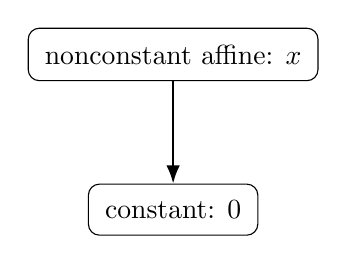
\begin{tikzpicture}[>=Latex,node distance=1.3cm]
  \node (x) [draw,rounded corners,inner sep=6pt] {nonconstant affine: \(x\)};
  \node (c) [draw,rounded corners,inner sep=6pt,below=of x] {constant: \(0\)};
  \draw[->,thick] (x) -- (c);
\end{tikzpicture}
\end{center}
The two core concepts---equivalence class and degeneration order---came from
the same implementation rule.

\subsection*{Second example: quadratic maps
\texorpdfstring{\(\F_3\to\F_3\)}{F3 to F3}}

Every degree-at-most-two polynomial over \(\F_3\) is uniquely a function of
the form \(ax^2+bx+c\).  Invertible affine changes of input and output give
three classes:
\[
  0,\qquad x,\qquad x^2.
\]
Their class sizes are \(3,6,18\), respectively, accounting for all
\(3^3=27\) quadratic polynomial functions of one variable.
Both nonconstant classes implement a constant.  Neither implements the other:
a nonconstant affine substitution preserves the degree of \(x^2\), while a
singular substitution is constant.  The poset branches:
\begin{center}
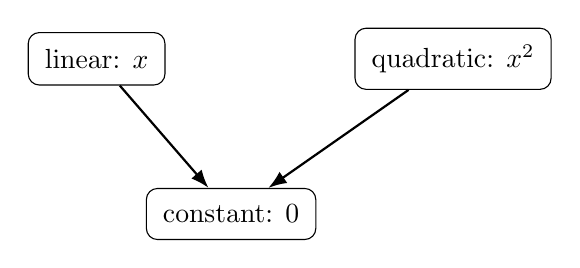
\begin{tikzpicture}[>=Latex,node distance=1.5cm and 2.4cm]
  \node (l) [draw,rounded corners,inner sep=6pt] {linear: \(x\)};
  \node (q) [draw,rounded corners,inner sep=6pt,right=of l] {quadratic: \(x^2\)};
  \node (c) [draw,rounded corners,inner sep=6pt,below right=1.3cm and -0.25cm of l] {constant: \(0\)};
  \draw[->,thick] (l) -- (c);
  \draw[->,thick] (q) -- (c);
\end{tikzpicture}
\end{center}
This is the first warning that ``more complicated'' is not automatically a
linear ranking.  The linear and quadratic classes lose different structure.

\subsection*{Third example: quadratic maps
\texorpdfstring{\(\F_3^2\to\F_3\)}{F3 squared to F3}}

Now take
\[
  Q(x,y)=ax^2+bxy+cy^2+dx+ey+f.
\]
There are \(3^6=729\) coefficient vectors, but only six affine-equivalence
classes:
\[
  0,\quad x,\quad x^2,\quad x^2+y,\quad xy,\quad x^2+y^2.
\]
The last two are the split and anisotropic nonsingular quadratic forms.  The
split form has an isotropic line and can lose its quadratic part along that
line, producing \(x\).  The anisotropic form has no such line, so it reaches
\(x^2\) but not \(x\).  Figure~\ref{fig:q3-affine} later displays the full
six-node Hasse diagram with all class sizes.

This example already touches classical quadratic-form theory.  The framework
has not replaced the classical invariants; it has explained why they appear.
Rank, the radical, and isotropy are precisely the information that survives or
disappears under singular affine processors.

\subsection*{Why go projective?}

Translations mix homogeneous degrees.  If we want to study the leading part
of a polynomial, or what its fibers do at infinity, the natural next step is
to keep only homogeneous maps and use linear processors.  A homogeneous
scalar polynomial \(Q\in\Sym^d(V^*)\) scales by
\(Q(\lambda v)=\lambda^dQ(v)\), so its zero set descends to projective space
\(\mathbf P(V)\).

There is a small but important distinction.  A scalar form on \(V\) does
\emph{not} give an interesting map \(\mathbf P(V)\to\mathbf P(K)\), because
\(\mathbf P(K)=\mathbf P^0\) is one point.  It is naturally a section of
\(\mathcal O(d)\), or equivalently a projective hypersurface \(Q=0\).  A tuple
\[
  F=(F_0,\ldots,F_r),\qquad F_i\in\Sym^d(V^*),
\]
does give a rational map
\[
  \mathbf P(V)\dashrightarrow\mathbf P^r,
  \qquad [v]\longmapsto[F_0(v):\cdots:F_r(v)].
\]
It is a total projective morphism exactly when the forms have no common
projective zero.  Thus scalar forms and tuples belong in the same tensor
framework, but their geometric readings are different.

Over \(\F_3\), binary quadratic forms have four classes:
\[
  0,\qquad x^2,\qquad xy,\qquad x^2+y^2.
\]
Their orbit sizes are respectively \(1,8,12,6\), summing to the
\(3^3=27\) formal binary quadratics.
The last two are different degree-two divisors on \(\mathbf P^1\): split over
\(\F_3\), or conjugate over \(\F_9\).  Their degeneration diagram is
\begin{center}
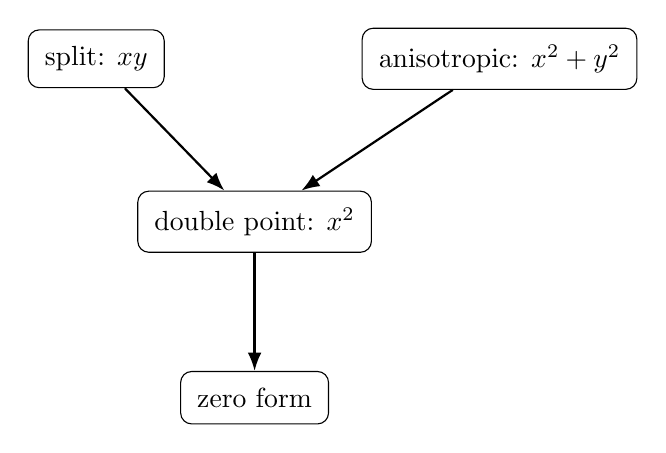
\begin{tikzpicture}[>=Latex,node distance=1.5cm and 2.5cm]
  \node (s) [draw,rounded corners,inner sep=6pt] {split: \(xy\)};
  \node (a) [draw,rounded corners,inner sep=6pt,right=of s] {anisotropic: \(x^2+y^2\)};
  \node (r) [draw,rounded corners,inner sep=6pt,below right=1.3cm and -0.35cm of s] {double point: \(x^2\)};
  \node (z) [draw,rounded corners,inner sep=6pt,below=of r] {zero form};
  \draw[->,thick] (s) -- (r);
  \draw[->,thick] (a) -- (r);
  \draw[->,thick] (r) -- (z);
\end{tikzpicture}
\end{center}
Pairs of binary quadratics give rational self-maps
\(\mathbf P^1\dashrightarrow\mathbf P^1\).  Their seven classes and eight
Hasse covers appear in Figure~\ref{fig:q3-p1-tensors}; the base-point-free
nodes are genuine quadratic morphisms.  Ternary quadratic forms similarly
give projective conics in \(\mathbf P^2\), with five classes.  These examples
will be drawn in Section~\ref{sec:beyond-quadratic}.

We now return to the general story.  Depending on the processor class, the
same implementation equation appears as a reduction in complexity theory, a
simulation in information theory, a restriction of tensors, or a left--right
action in singularity theory.  The point is to keep the equation fixed and
vary the processors deliberately.

The next continuation is where the companion paper
\cite{vorozhtsov-exchange} enters.  For finite maps with a fiber-preserving
processor convention, the asymptotic exchange rate is computed exactly from
the partition functions
\[
  Z_f(\beta)=\sum_y |f^{-1}(y)|^\beta.
\]
Many polynomial classes have the same fiber signature, while others do not,
so this produces a second numerical geometry on the class poset.  It is a
useful observer, but it must not be confused with the block-affine exchange
rate.  The two processor classes are different.

The paper has three levels of certainty.

\begin{enumerate}
  \item The processor preorder, the quadratic normal forms, the finite-field
  class counts, and the no-arbitrage theorem are proved or reduced to standard
  quadratic-form calculations.
  \item The larger homogeneous and cubic diagrams, and the displayed exchange
  matrices, are reproducible finite computations.
  \item The possible relation among exchange matrices, local zeta profiles,
  Weil positivity, and the Riemann hypothesis is exploratory.  We state
  precisely what is known and what is not connected.
\end{enumerate}

This separation is part of the contribution.  It prevents a suggestive common
vocabulary---resources, partition functions, spectra, exchange matrices---from
being mistaken for a theorem that has not yet been found.

\section{Processors, equivalence, and order}
\label{sec:processors}

Fix a field \(K\), dimensions \(n,m\), and a degree bound \(d\).  Write
\[
  \Pol_d(K^n,K^m)
\]
for polynomial maps of total degree at most \(d\).  An affine input processor
and output processor have the form
\[
  a(x)=Ax+t,
  \qquad
  b(y)=By+u,
\]
with \(A\in\operatorname{Mat}_{n\times n}(K)\) and
\(B\in\operatorname{Mat}_{m\times m}(K)\).

\begin{definition}[Affine implementation]
For \(f,g\in\Pol_d(K^n,K^m)\), say that \(g\) implements \(f\), and write
\(f\impl_{\rm aff}g\), when
\begin{equation}
  f=b\circ g\circ a
  \label{eq:affine-implementation}
\end{equation}
for affine \(a\) and \(b\).  The matrices \(A\) and \(B\) may be singular,
including zero.
\end{definition}

The convention is that the resource is on the right of \(\impl_{\rm aff}\):
an arrow in a Hasse diagram points from \(g\) down to a map \(f\) that it
implements.

\begin{proposition}
Affine implementation is a preorder.
\end{proposition}

\begin{proof}
Identity processors prove reflexivity.  If
\(f=b_1\circ g\circ a_1\) and \(g=b_2\circ h\circ a_2\), then
\[
  f=(b_1\circ b_2)\circ h\circ(a_2\circ a_1),
\]
and affine maps are closed under composition.
\end{proof}

Invertible processors define the affine left--right equivalence relation
\begin{equation}
  f\simaff g
  \quad\Longleftrightarrow\quad
  f=b\circ g\circ a,
  \qquad a\in\Aff_n(K),\ b\in\Aff_m(K)
  \text{ invertible}.
  \label{eq:affine-equivalence}
\end{equation}
This is the finite-dimensional affine version of the left--right equivalence
used for map germs and singularities; see, for example,
\cite{kerner-left-right}.  The set \(\Pol_d(K^n,K^m)\) is a representation
space for the invertible affine group, and its equivalence classes are group
orbits.

Singular processors induce a directed relation on those orbits.  In every
quadratic diagram below this relation is antisymmetric.  In general it need
not be: if two different invertible orbits are mutually reachable using
singular processors, one must contract the strongly connected component.
The quotient by mutual reachability is always a poset.

\begin{remark}[Exact reachability versus orbit closure]
Our arrows solve the exact equation \eqref{eq:affine-implementation} with
possibly singular processors.  This is related to, but not automatically the
same as, containment of algebraic-group orbit closures.  Orbit-closure theory
allows limits of invertible transformations and is governed by results such
as \cite{birkes-orbits}; an exact singular factorization is a more specific
certificate.  The two orders should not be identified without proof.
\end{remark}

\begin{remark}[Bounded-degree nonlinear processors]
If input processors have degree at most two, a one-step relation is generally
not transitive because two quadratic substitutions may compose to degree
four.  The correct object is then the transitive closure of allowed steps,
followed by quotienting mutual reachability.  This distinction explains the
large collapse in the cubic \(\F_3\) example of
Section~\ref{sec:beyond-quadratic}.
\end{remark}

The implementation order comes with immediate monotones: polynomial degree,
the dimension of the affine span of the image, coordinate rank for homogeneous
tensors, and appropriate ranks of derivatives or polar forms cannot increase
under the corresponding processors.  These monotones help prove that proposed
arrows are Hasse covers and that omitted arrows are impossible.

\section{Cartesian powers and the operational rate}
\label{sec:rates}

For \(f:K^n\to K^m\), let
\[
  f^{\times r}:K^{nr}\longrightarrow K^{mr},
  \qquad
  f^{\times r}(x_1,\ldots,x_r)
  =(f(x_1),\ldots,f(x_r)).
\]
The block processor is allowed to mix the \(r\) copies.  Define
\[
  k_{g\to f}(r)
  =\max\{k:f^{\times k}\impl_{\rm aff}g^{\times r}\}.
\]
Block-diagonal composition gives
\(k(r+s)\ge k(r)+k(s)\), so Fekete's lemma gives the limit
\begin{equation}
  \caff(g\to f)
  =\lim_{r\to\infty}\frac{k_{g\to f}(r)}r
  =\sup_{r\ge1}\frac{k_{g\to f}(r)}r,
  \label{eq:affine-rate}
\end{equation}
with infinite values permitted for degenerate resources.

The same construction works for any processor family that is closed under
composition and block sum.  The following consequence is the fundamental
``no-arbitrage'' statement.

\begin{theorem}[Composition and no arbitrage]
Let \(C(i\to j)\) be operational asymptotic rates in such a resource theory.
Then
\begin{equation}
  C(i\to j)C(j\to k)\le C(i\to k).
  \label{eq:multiplicative-triangle}
\end{equation}
For normalized nondegenerate resources with \(C(i\to i)=1\), every directed
cycle \(\mathcal C=(i_0,i_1,\ldots,i_{\ell}=i_0)\) satisfies
\begin{equation}
  R(\mathcal C)
  :=\prod_{r=0}^{\ell-1}C(i_r\to i_{r+1})\le1.
  \label{eq:no-arbitrage-cycle}
\end{equation}
\end{theorem}

\begin{proof}
Choose block conversions with rates arbitrarily close to
\(C(i\to j)\) and \(C(j\to k)\), clear the block denominators, and compose
them.  This realizes any rate strictly below their product from \(i\) to
\(k\), proving \eqref{eq:multiplicative-triangle}.  Iterating around a cycle
gives \(R(\mathcal C)\le C(i_0\to i_0)=1\).
\end{proof}

For a finite collection put \(M_{ij}=C(i\to j)\).  When all entries are
positive, the logarithmic costs
\begin{equation}
  a_{ij}=-\log M_{ij}
  \label{eq:log-cost}
\end{equation}
satisfy the directed triangle inequality
\[
  a_{ik}\le a_{ij}+a_{jk}
\]
and every directed cycle has nonnegative total cost.  The costs need not be
nonnegative edge by edge because one resource may produce more than one copy
of another; it is the cycle sum that cannot be negative.

\subsection{Why no arbitrage does not imply positive semidefiniteness}

The matrix \(M\) is directed and normally nonsymmetric, so positive
semidefiniteness is not even an intrinsic property of it.  More strongly,
entrywise positivity, unit diagonal, and all cycle inequalities do not imply
positive semidefiniteness even after symmetry is imposed.  For example,
\[
  S=
  \begin{pmatrix}
    1&0.9&0.9\\
    0.9&1&0.1\\
    0.9&0.1&1
  \end{pmatrix}.
\]
Every cycle product is at most one, but
\[
  \det S
  =1+2(0.9)(0.9)(0.1)-0.9^2-0.9^2-0.1^2
  =-0.468<0.
\]
Thus the no-arbitrage cone and the positive-semidefinite cone are genuinely
different geometries.

\section{Quadratic maps \texorpdfstring{\(K^2\to K\)}{K2 to K}}
\label{sec:quadratic-normal-forms}

Consider
\begin{equation}
  Q(x,y)=ax^2+bxy+cy^2+dx+ey+f.
  \label{eq:binary-quadratic}
\end{equation}
For \(\operatorname{char}K\ne2\), write
\[
  Q(z)=z^{\mathsf T}Sz+\ell^{\mathsf T}z+c
\]
with \(S\) symmetric.  Translation by \(t\) replaces the linear part by
\(\ell+2St\).  Hence the component of \(\ell\) in the image of \(S\) can be
removed.  What remains is a linear functional on the radical of \(S\).
This gives four preliminary types:
\[
  \text{constant},\qquad
  x,\qquad
  x^2,\qquad
  x^2+y,
\]
followed by the similarity classes of nonsingular binary quadratic forms.

The form \(x^2+y\) is called parabolic here.  Its linear term lives along the
radical of its quadratic part, and no translation removes it.  A nonsingular
binary form has no radical, so every linear term can be removed.

Under a singular input matrix, a nondegenerate form always restricts to a
rank-one form \(x^2\).  It restricts to a nonconstant linear map exactly when
it has an isotropic direction: choosing that direction kills the quadratic
term while a translation in a transverse direction creates the linear term.
This one observation determines the split/anisotropic difference in every
diagram below.

\begin{theorem}[Odd finite fields]
For every odd prime power \(q\), affine equivalence on degree-at-most-two maps
\(\F_q^2\to\F_q\) has six classes:
\[
  1,\quad x,\quad x^2,\quad x^2+y,\quad xy,\quad x^2-\nu y^2,
\]
where \(\nu\) is a nonsquare.  Their numbers of coefficient vectors are
\begin{center}
\begin{tabular}{@{}lr@{}}
\toprule
type & class size\\
\midrule
constant & \(q\)\\
linear & \(q(q^2-1)\)\\
rank-one quadratic & \(q^2(q^2-1)\)\\
parabolic & \(q^2(q-1)(q^2-1)\)\\
split quadratic & \(q^4(q^2-1)/2\)\\
anisotropic quadratic & \(q^4(q-1)^2/2\)\\
\bottomrule
\end{tabular}
\end{center}
The Hasse covers are
\begin{align*}
  [x^2+y]&\longrightarrow[x],\ [x^2],\\
  [xy]&\longrightarrow[x],\ [x^2],\\
  [x^2-\nu y^2]&\longrightarrow[x^2],\\
  [x],\ [x^2]&\longrightarrow[1].
\end{align*}
\end{theorem}

\begin{proof}[Proof sketch]
The preceding translation argument gives the four singular types.  The usual
Witt classification of nonsingular binary forms over \(\F_q\) gives one split
and one anisotropic similarity class; see \cite{lam-quadratic,lidl-finite-fields}.
The arrows follow from rank-one restrictions and isotropy.  Orbit--stabilizer
counts give the displayed sizes, which sum to \(q^6\).
\end{proof}

Figure~\ref{fig:q3-affine} is the case \(q=3\).  Its six class sizes are
\(3,24,72,144,324,162\), summing to \(3^6=729\).

\begin{figure}[t]
  \centering
  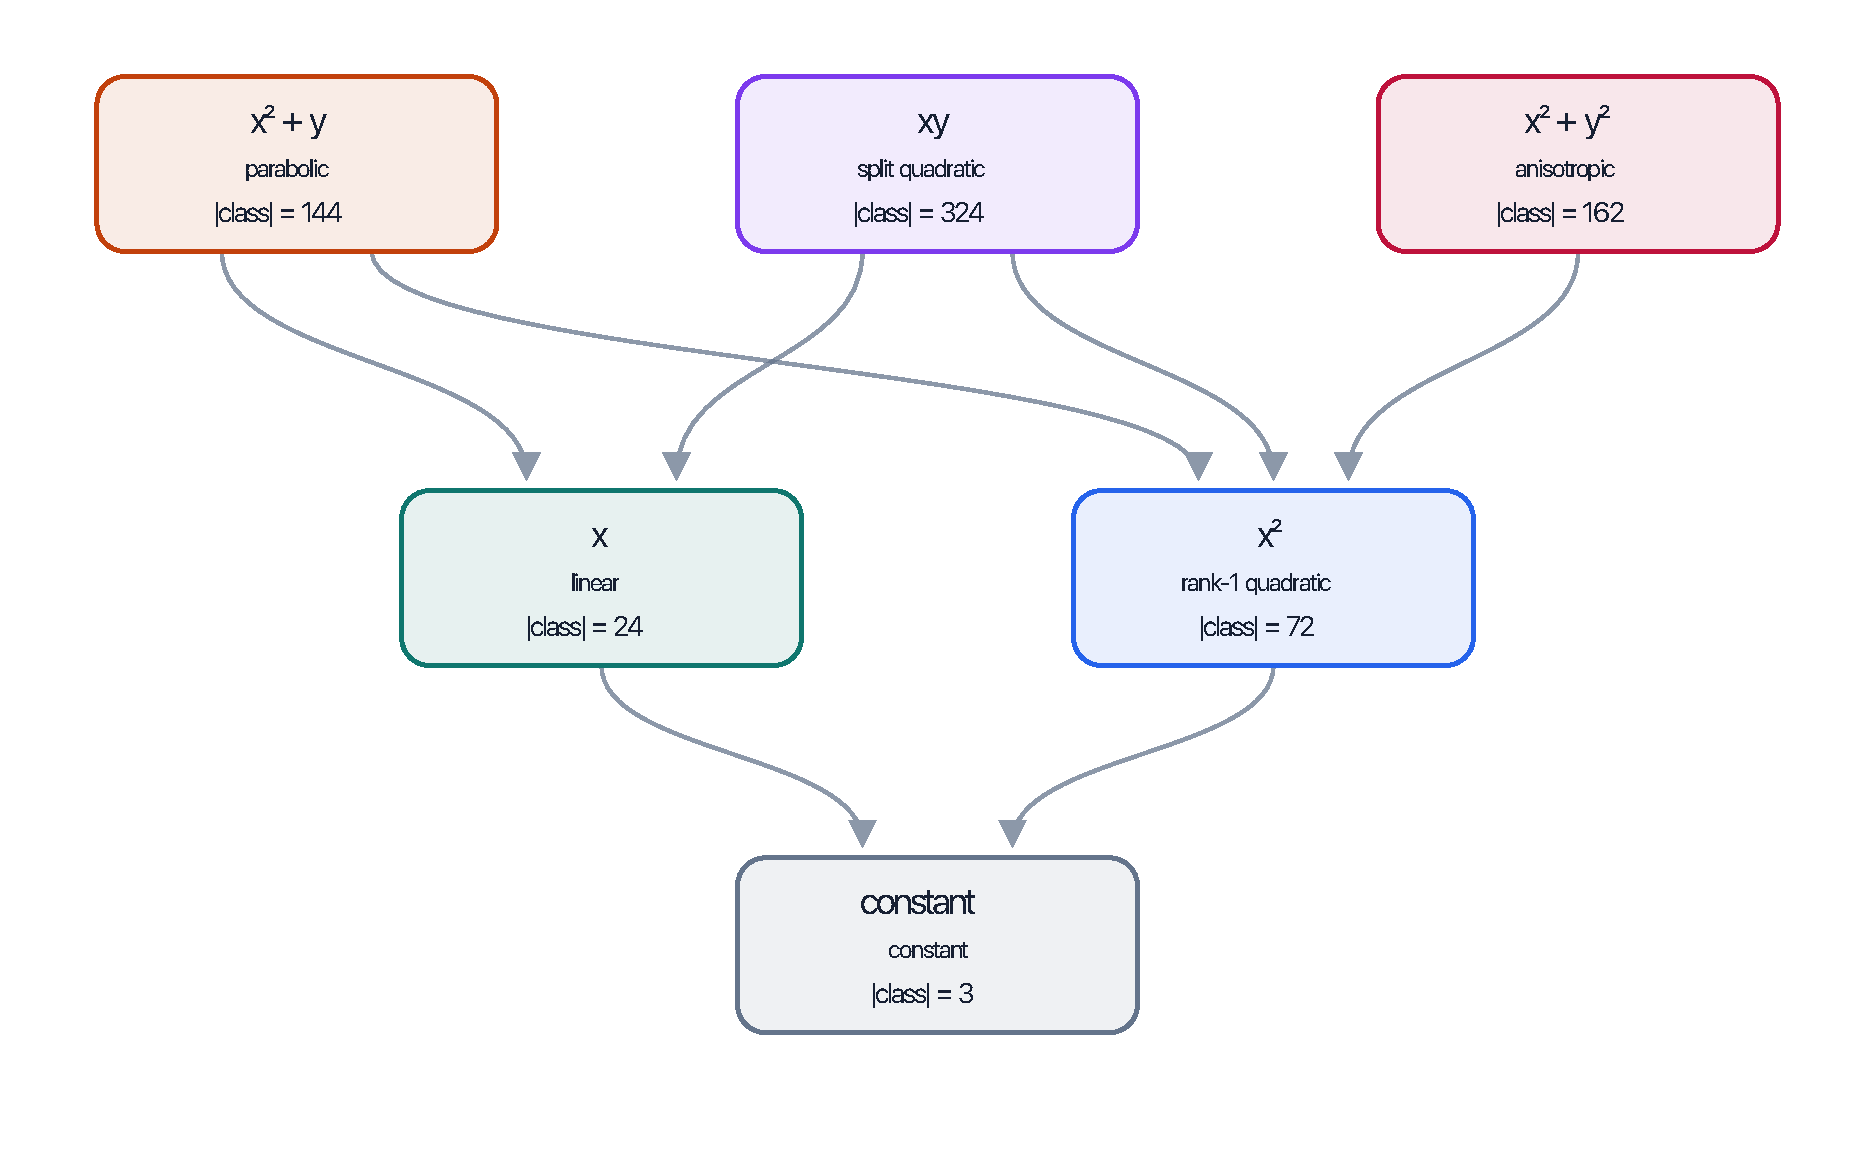
\includegraphics[width=0.88\textwidth]{figures/quadratic-map-poset-q3.pdf}
  \caption{The affine-processor Hasse diagram for quadratic maps
  \(\F_3^2\to\F_3\): six classes and seven covers.  Singular affine input
  and output processors are allowed.  Arrows point from a resource map to an
  immediately implementable degeneration; class sizes count coefficient
  vectors.}
  \label{fig:q3-affine}
\end{figure}

\subsection{Characteristic two}

In characteristic two the polar bilinear form no longer determines the
quadratic form, and square terms behave additively.  Over \(\F_2\), polynomial
functions satisfy \(x^2=x\) and \(y^2=y\), leaving only three classes:
constant, balanced linear, and weight-one-or-three, represented by \(1,x,xy\).

For even \(q\ge4\), there are seven classes.  In addition to the constant,
linear, pure-square, parabolic, split, and anisotropic classes, there is an
aligned-linear class \(x^2+x\).  With
\(\delta\in\F_q\) satisfying \(\operatorname{Tr}_{\F_q/\F_2}(\delta)=1\),
the nonsingular representatives are \(xy\) and
\(x^2+xy+\delta y^2\).  The class sizes are
\begin{center}
\begin{tabular}{@{}lr@{}}
\toprule
type & class size\\
\midrule
constant & \(q\)\\
linear & \(q(q^2-1)\)\\
pure square & \(q(q^2-1)\)\\
square plus aligned linear & \(q(q-1)(q^2-1)\)\\
parabolic & \(q^2(q-1)(q^2-1)\)\\
split quadratic & \(q^4(q^2-1)/2\)\\
anisotropic quadratic & \(q^4(q-1)^2/2\).\\
\bottomrule
\end{tabular}
\end{center}
Again the sum is \(q^6\).  The trace/Arf invariant replaces the discriminant
test.  The aligned-linear node is incomparable with the pure-square and
ordinary linear nodes, although all three degenerate to a constant.

\section{Changing the field}
\label{sec:fields}

The processor definition does not change with the field; only the quadratic
similarity classes and isotropic directions change.

\subsection{The real and complex numbers}

Over \(\C\), every nonsingular binary quadratic form is similar to \(xy\), so
the diagram has five nodes.  Over \(\R\), output rescaling identifies positive
and negative definite forms, leaving two nonsingular classes: the indefinite
form \(xy\) and the definite form \(x^2+y^2\).  The real diagram therefore has
six nodes.  The definite class has no arrow to \(x\), exactly because it has no
real isotropic direction.

All nonempty real or complex orbits have continuum cardinality.  Orbit
dimension is the useful label: constant, linear, rank-one, parabolic, and open
nonsingular strata have dimensions \(1,3,4,5,6\), respectively, over the base
field.  These are real dimensions for \(\R\) and complex dimensions for
\(\C\).

\begin{figure}[t]
  \centering
  \begin{minipage}[t]{0.49\textwidth}
    \centering
    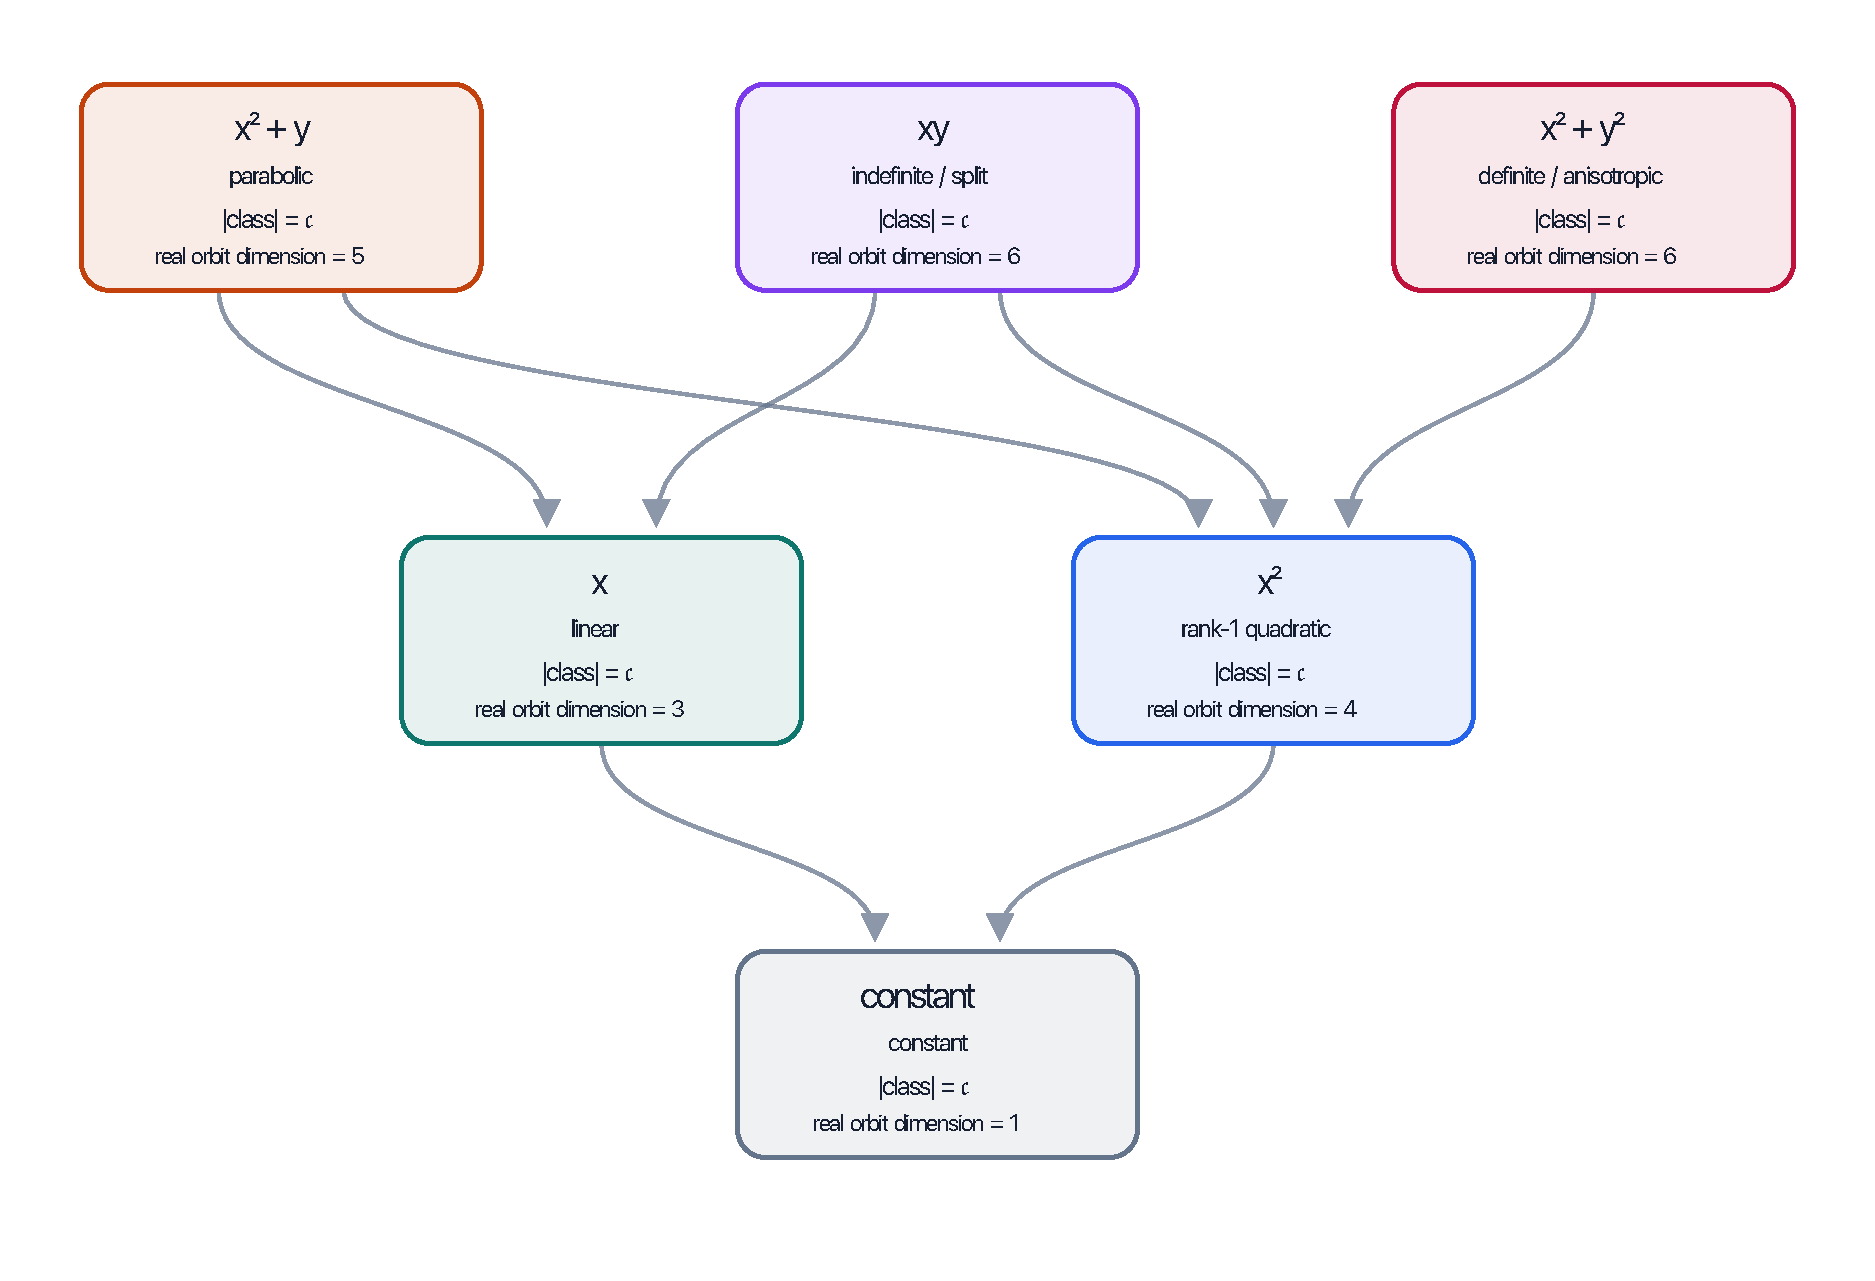
\includegraphics[width=\textwidth]{figures/quadratic-map-poset-R.pdf}
  \end{minipage}
  \hfill
  \begin{minipage}[t]{0.49\textwidth}
    \centering
    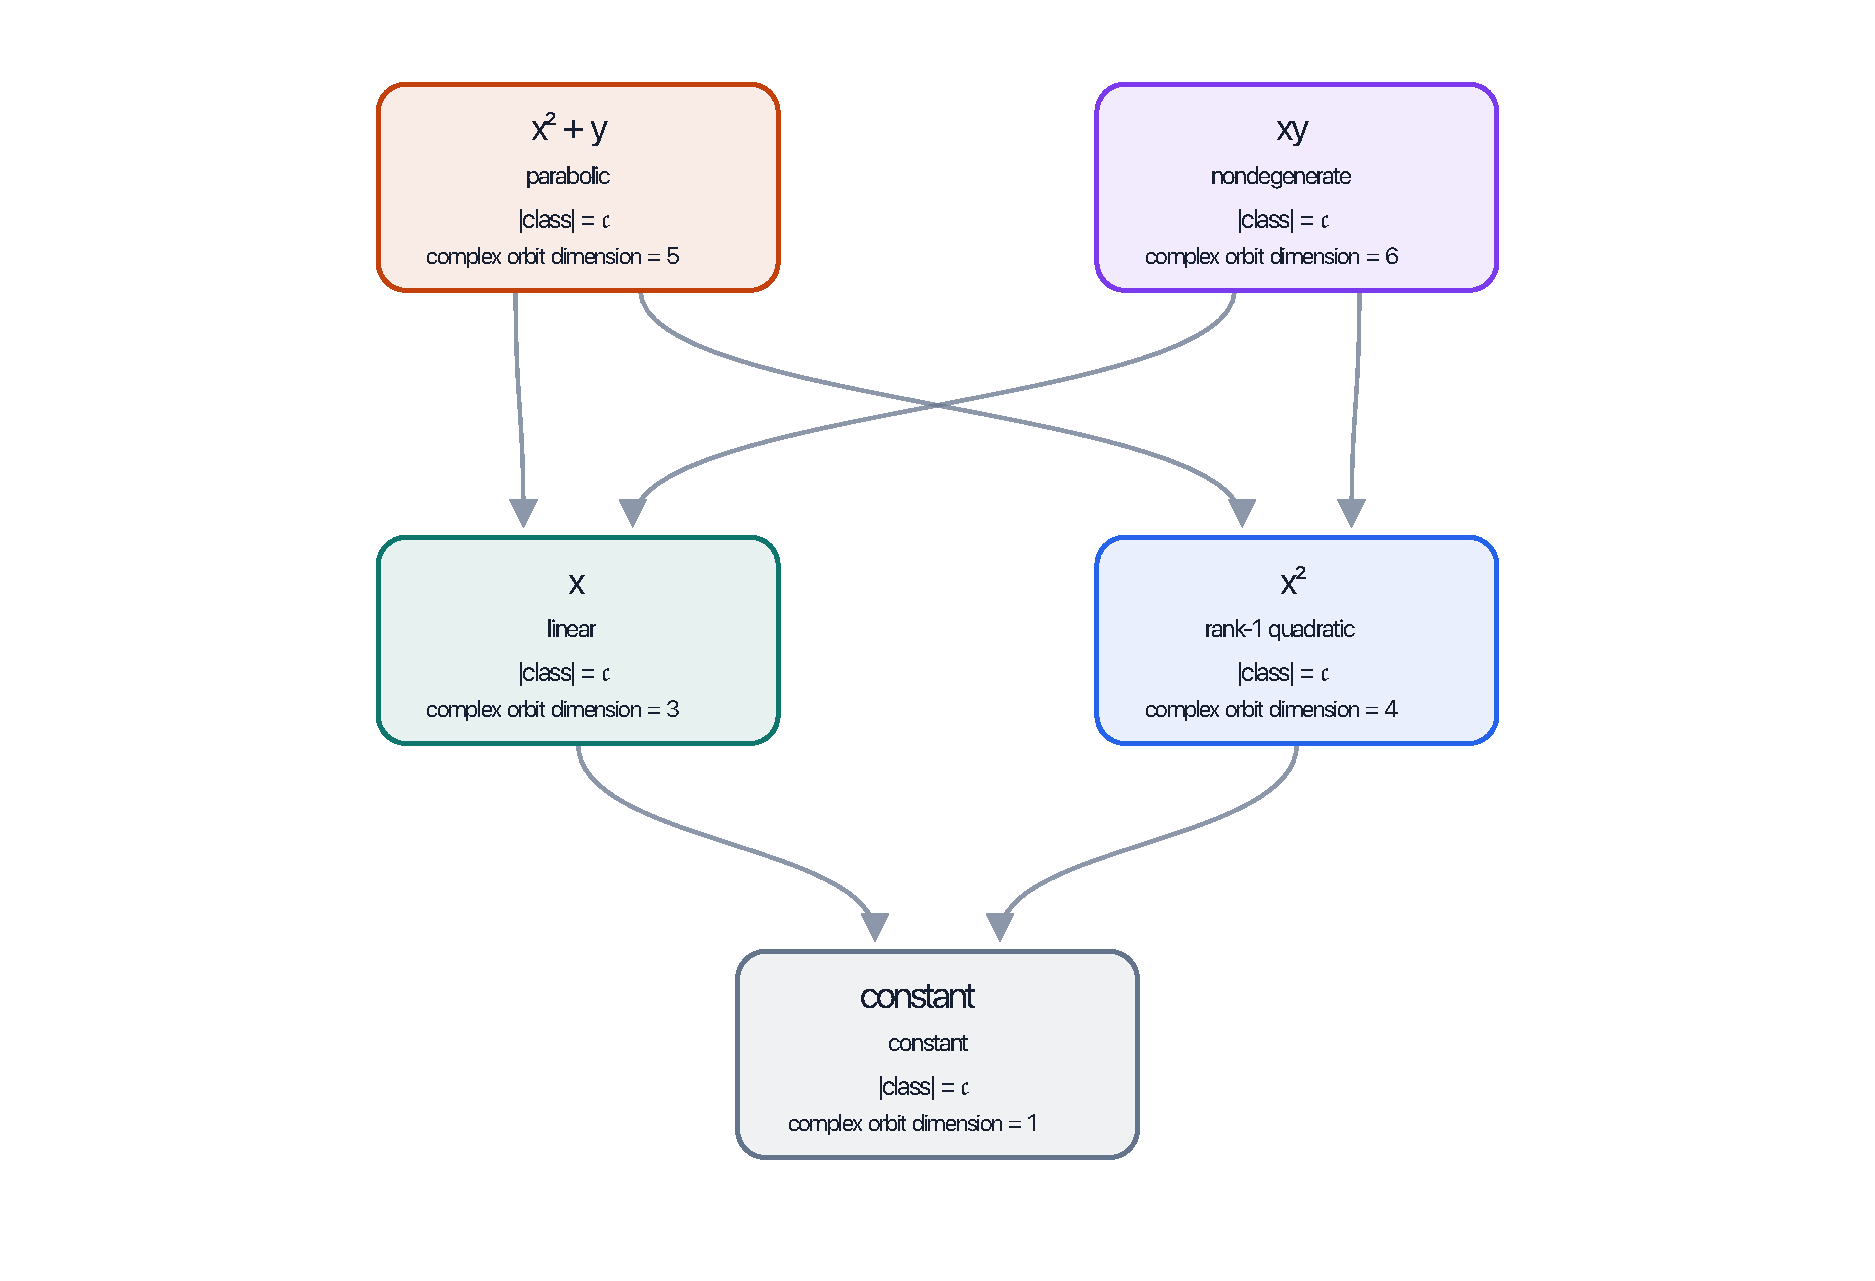
\includegraphics[width=\textwidth]{figures/quadratic-map-poset-C.pdf}
  \end{minipage}
  \caption{The same affine implementation convention over \(\R\) and \(\C\).
  The real diagram has six classes and seven covers; the complex diagram has
  five classes and six covers.  Singular affine input and output processors
  are allowed.  The field changes the nonsingular quadratic-form classes, not
  the definition of the order.}
  \label{fig:real-complex}
\end{figure}

\subsection{Local fields}

For a non-Archimedean local field, the square-class group creates several
nonsingular binary forms.  Over \(\Q_3\), the representatives
\(d\in\{1,-1,3,-3\}\) in
\[
  x^2+d y^2
\]
give one split class \(d=-1\) and three pairwise-incomparable anisotropic
classes.  Together with the four singular types, this gives eight nodes.

\begin{figure}[t]
  \centering
  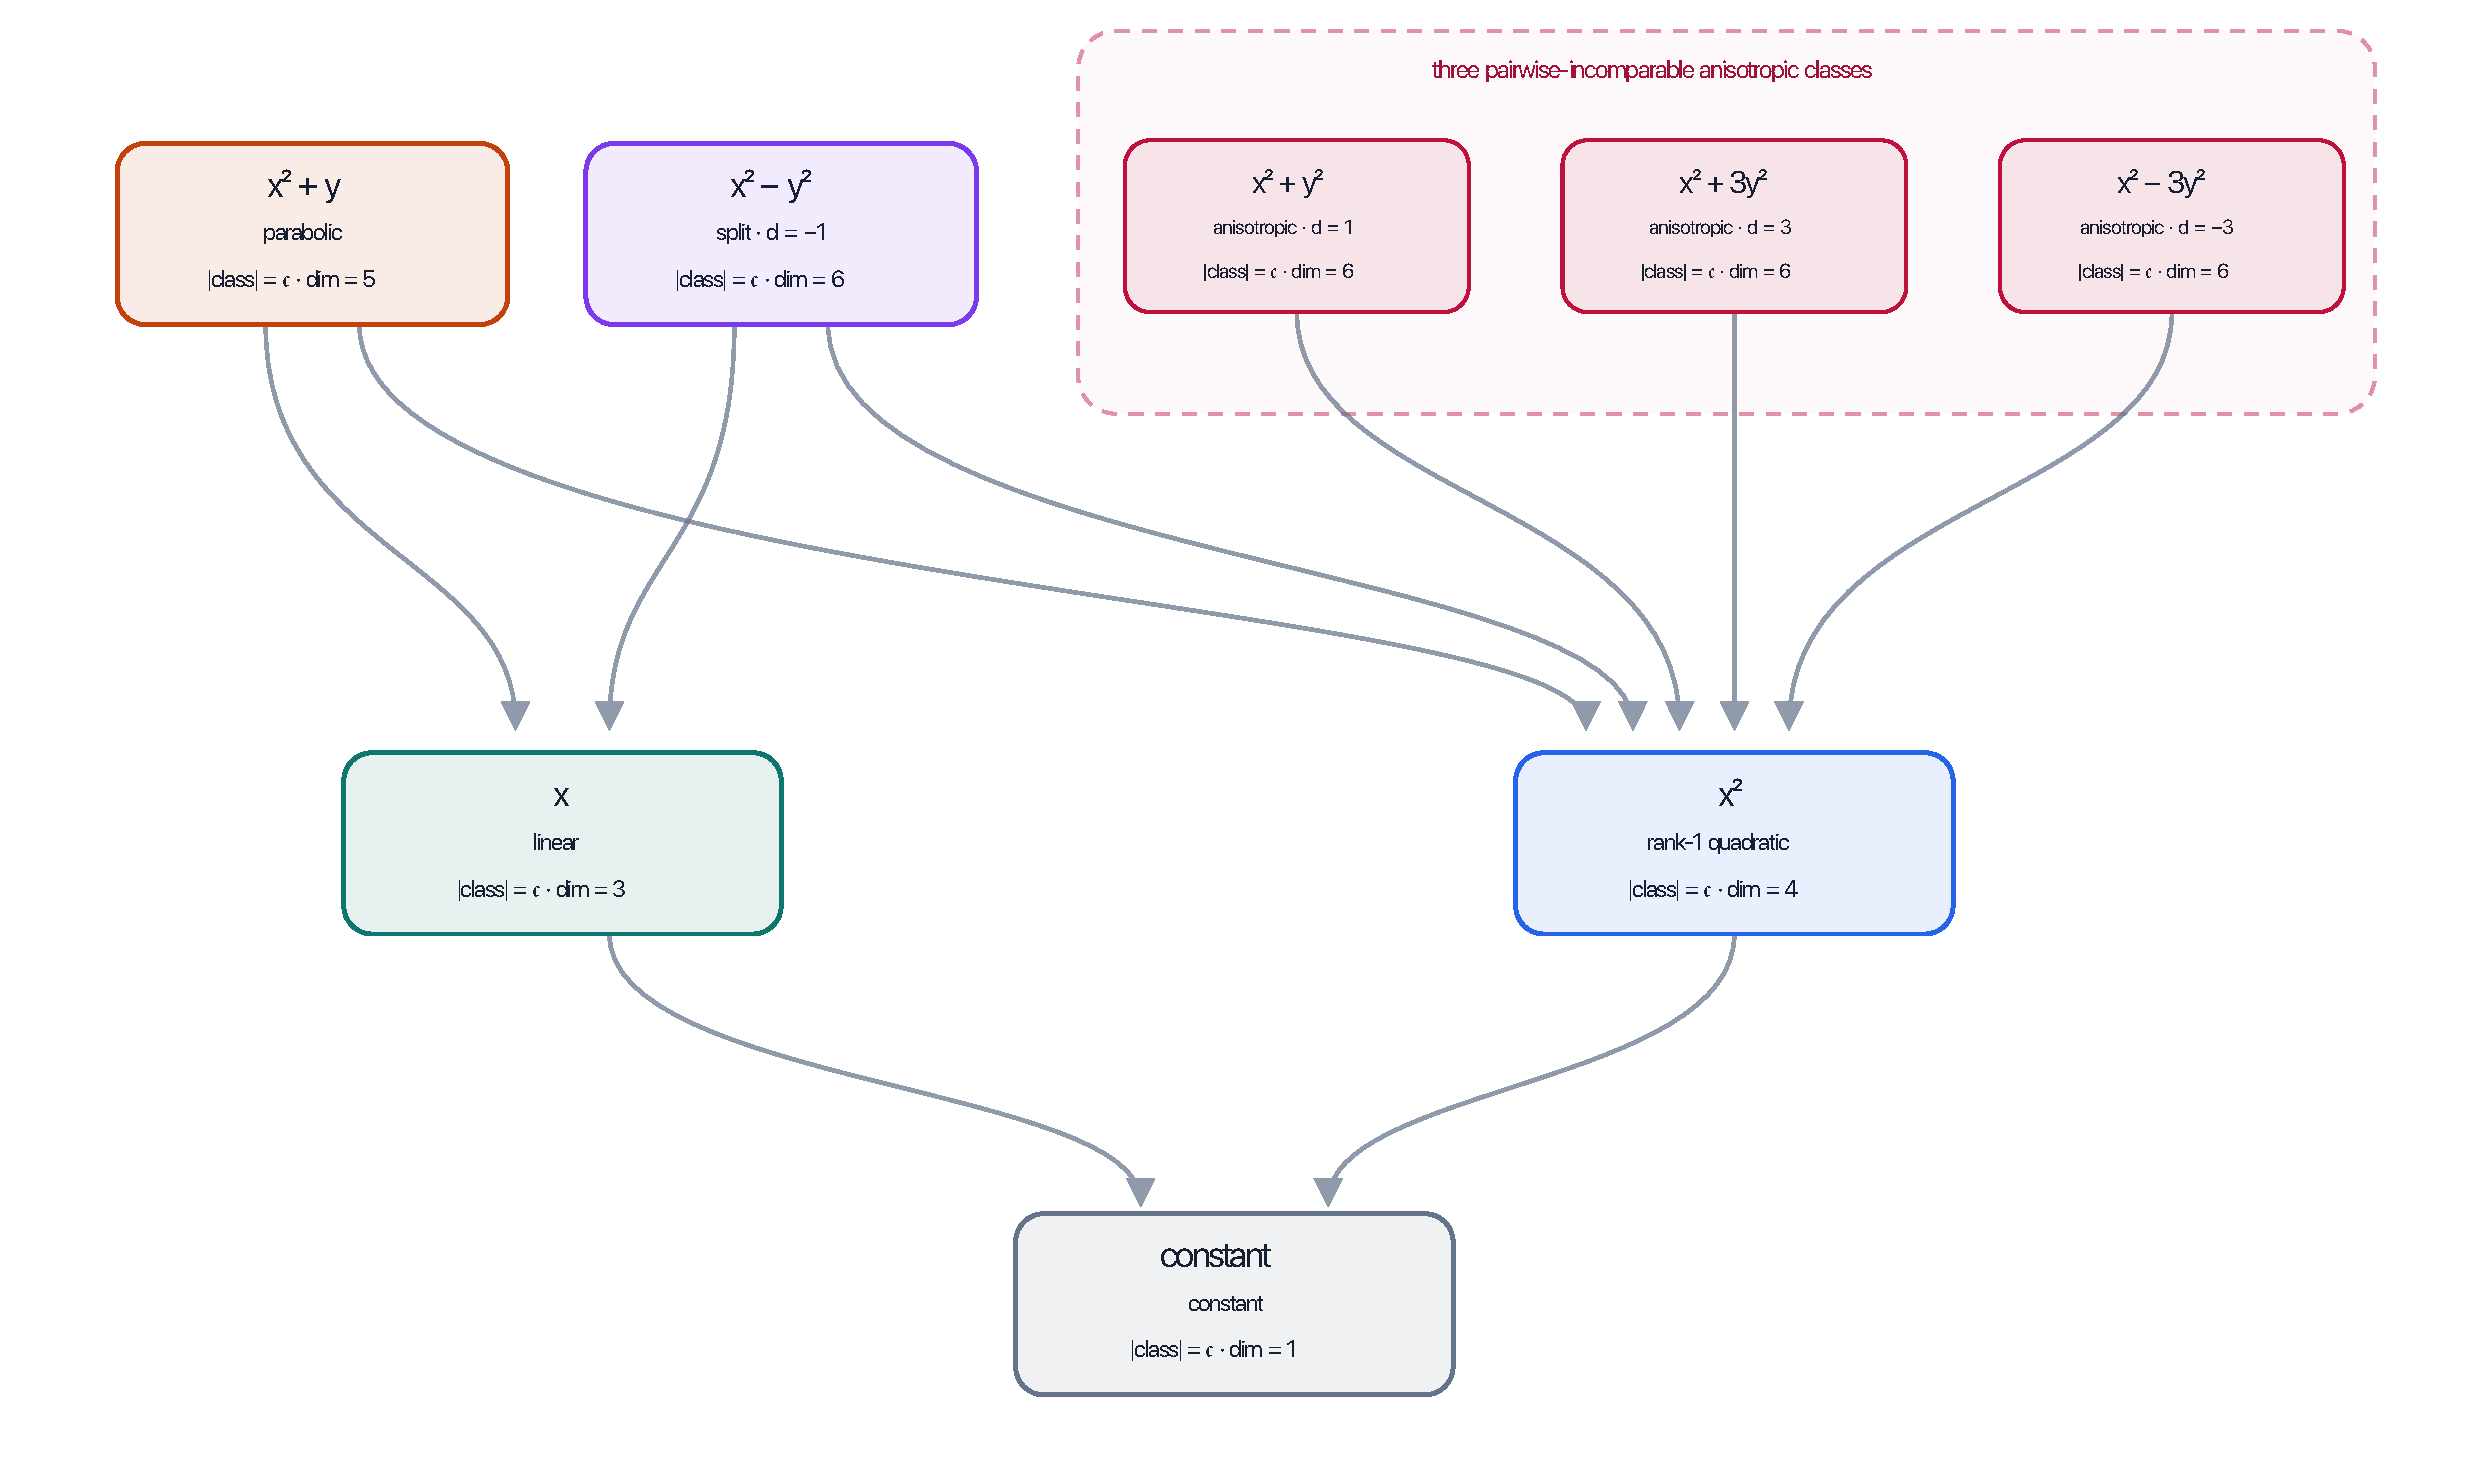
\includegraphics[width=0.92\textwidth]{figures/quadratic-map-poset-q3-adic.pdf}
  \caption{Quadratic maps \(\Q_3^2\to\Q_3\) with singular affine processors:
  eight classes and nine covers.  The three anisotropic square classes are
  incomparable and have no arrow to the linear node.}
  \label{fig:q3-adic}
\end{figure}

Over \(\Q_2\), the square classes
\[
  \{1,-1,2,-2,5,-5,10,-10\}
\]
give one split and seven anisotropic classes, hence twelve nodes.  Every
anisotropic node reaches \(x^2\) but not \(x\), and the seven are pairwise
incomparable in the one-shot affine poset.  Figure~\ref{fig:q2-adic} displays
the result.

\begin{figure}[t]
  \centering
  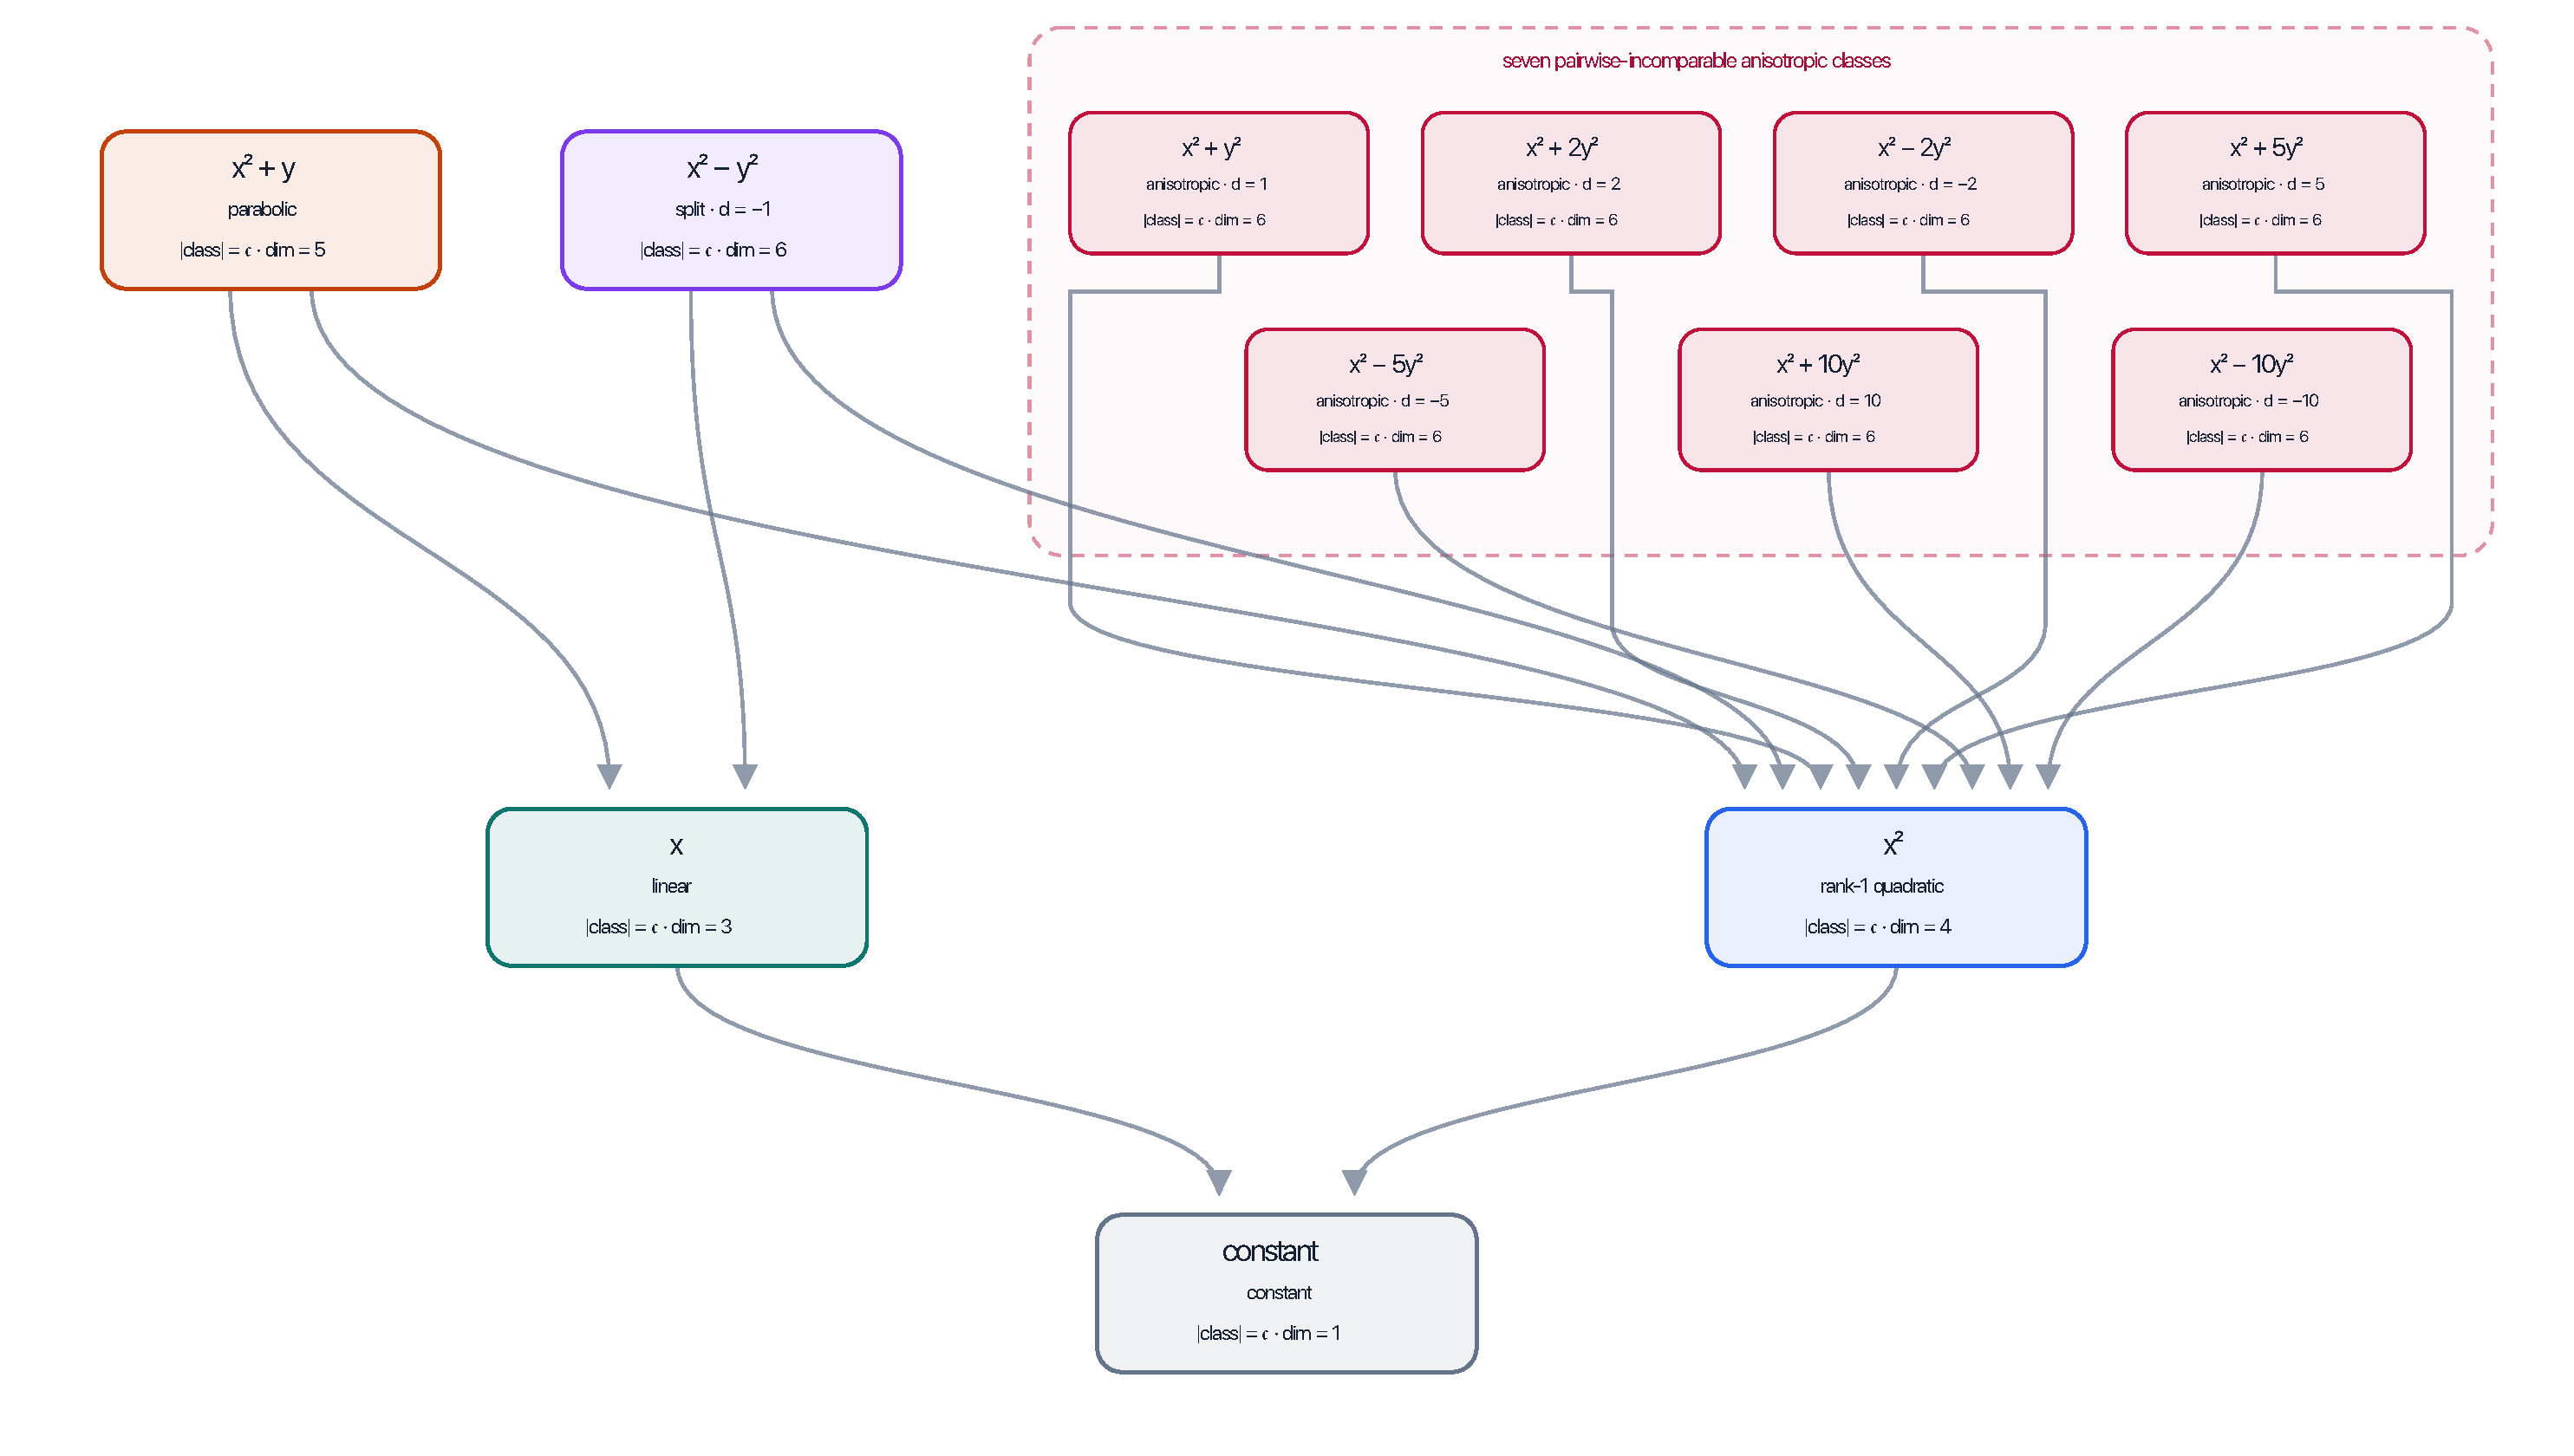
\includegraphics[width=0.96\textwidth]{figures/quadratic-map-poset-q2-adic.pdf}
  \caption{Quadratic maps \(\Q_2^2\to\Q_2\) with singular affine processors:
  twelve classes and thirteen covers.  Seven anisotropic classes sit above
  the rank-one node.  Their one-shot incomparability is exact; their
  block-affine exchange rates are largely unknown.}
  \label{fig:q2-adic}
\end{figure}

The orbit dimension labels are again \(1,3,4,5,6\) in the six-dimensional
coefficient space.  Cardinality cannot distinguish the orbits because every
class has continuum size.

\section{Beyond scalar quadratic maps}
\label{sec:beyond-quadratic}

The same construction applies to homogeneous tensors
\[
  F\in\operatorname{Hom}(\Sym^dV,W),
  \qquad
  G=B\circ F\circ A.
\]
Here translations are removed to preserve homogeneity.  Invertible
\(A\in\GL(V)\), \(B\in\GL(W)\) define equivalence; arbitrary linear maps
define degeneration.

Exhaustive calculations over \(\F_3\) give the following atlas.
\begin{center}
\begin{tabular}{@{}lrrr@{}}
\toprule
tensor family & total tensors & classes & Hasse covers\\
\midrule
ternary quadratic forms & \(3^6\) & 5 & 5\\
quadratic \(\F_3^2\to\F_3^2\) & \(3^6\) & 7 & 8\\
quadratic \(\F_3^3\to\F_3^3\) & \(3^{18}\) & 50 & 210\\
ternary cubic forms & \(3^{10}\) & 26 & 66\\
cubic \(\F_3^2\to\F_3^2\) & \(3^8\) & 19 & 32\\
\bottomrule
\end{tabular}
\end{center}
The quadratic \(3\)-input, \(3\)-output calculation quotients output changes
first, replacing coordinate tuples by subspaces of the six-dimensional space
of ternary quadrics.  Only \(45{,}256\) subspaces of dimension at most three
need be enumerated instead of all \(3^{18}\) tensors.

The first row of the table is the projective-conic example promised in the
introduction.  A ternary quadratic form is a section on \(\mathbf P^2\); its
zero locus is the whole plane for the zero form, a double line, two lines, an
anisotropic rank-two conic, or a nonsingular conic.  Singular linear input
processors contract these projective configurations exactly as shown in
Figure~\ref{fig:q3-ternary-forms}.

\begin{figure}[t]
  \centering
  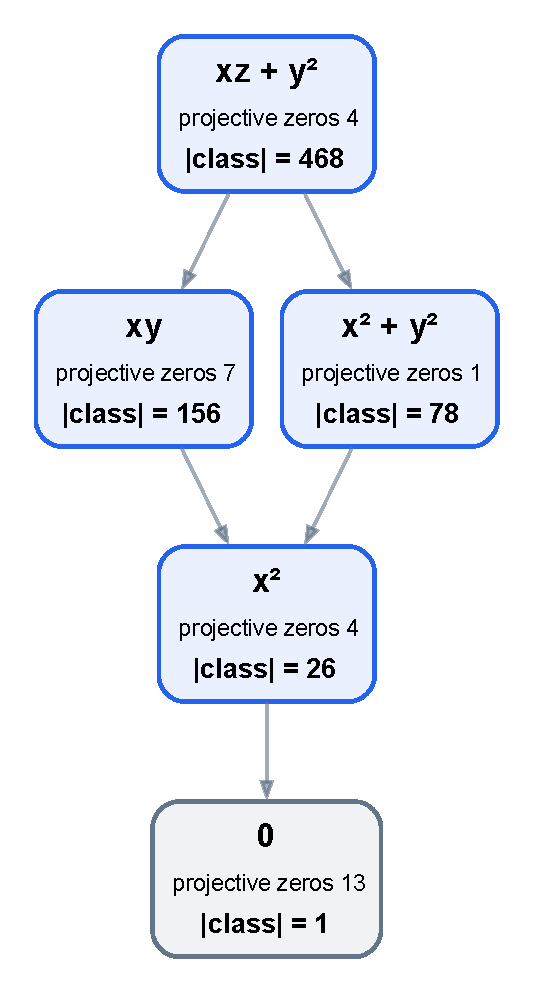
\includegraphics[width=0.88\textwidth,height=0.62\textheight,keepaspectratio]{figures/homogeneous-tensor-poset-q3-case1.pdf}
  \caption{Ternary quadratic forms over \(\F_3\), read as sections of
  \(\mathcal O(2)\) on \(\mathbf P^2\): five classes and five covers under
  possibly singular linear input processors and scalar output processors.
  The tensor classes are also five types of projective conic, including
  degenerate types.}
  \label{fig:q3-ternary-forms}
\end{figure}

\begin{figure}[t]
  \centering
  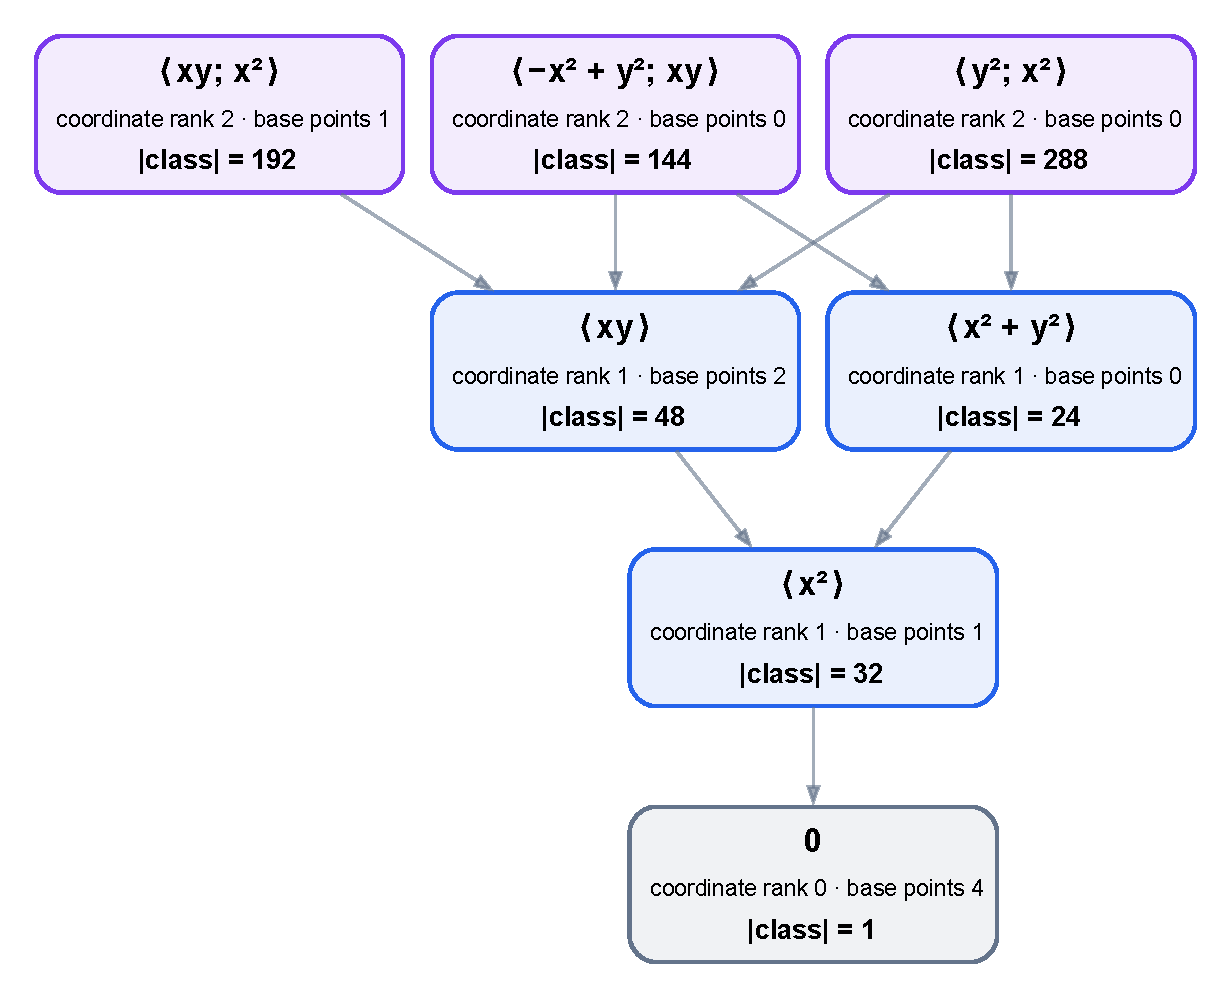
\includegraphics[width=0.94\textwidth]{figures/homogeneous-tensor-poset-q3-case2.pdf}
  \caption{Seven homogeneous quadratic tensor classes and eight covers for
  \(\F_3^2\to\F_3^2\), with possibly singular linear input and output
  processors.  This example will also carry a fiber-signature exchange matrix
  in Section~\ref{sec:signature-observer}.}
  \label{fig:q3-p1-tensors}
\end{figure}

\clearpage

For degree-at-most-three functions \(\F_3^2\to\F_3\), affine input and output
processors give \(14\) classes and \(22\) Hasse covers.  If quadratic input
processors are allowed and the generated preorder is used, the \(6{,}561\)
functions collapse to three mutual-reachability classes: surjective,
two-valued with fibers \(6+3\), and constant.

Over \(\F_8\), the functional identities responsible for this collapse no
longer hold.  Among \(8^{10}=1{,}073{,}741{,}824\) cubic functions, the
quadratic-input generated preorder has \(110\) classes.  The exact Hasse
diagram has \(23\) boxes after grouping order-theoretic twin antichains.  This
contrast is a warning: bounded-degree substitutions interact strongly with
the arithmetic of the field and with polynomial identities as functions.

\section{The fiber-signature observer}
\label{sec:signature-observer}

For a finite map \(f:X\to Y\), discard the labels and retain the nonzero fiber
sizes
\[
  \sigma(f)=(|f^{-1}(y_1)|,\ldots,|f^{-1}(y_r)|).
\]
The companion paper \cite{vorozhtsov-exchange} studies a processor convention
that injects each target fiber into an assigned source fiber.  For that
resource theory the exchange rate is
\begin{equation}
  \csig(g\to f)
  =\inf_{\beta\in[0,\infty]}
  \frac{\log Z_g(\beta)}{\log Z_f(\beta)},
  \qquad
  Z_f(\beta)=\sum_y|f^{-1}(y)|^\beta.
  \label{eq:signature-rate}
\end{equation}
Cartesian products multiply the partition functions, and the functions
\(Z_f(\beta)\) form the relevant asymptotic spectrum.  Equivalently,
\eqref{eq:signature-rate} is homothetic containment of Gibbs
energy--entropy regions.

\begin{remark}[No silent identification with the affine rate]
The affine and signature processors are not the same.  An affine input may be
singular, while the signature model preserves fibers by injections; conversely,
the signature model forgets all algebraic restrictions.  Therefore
\(\csig\) is used here as a computable observer attached to a polynomial map,
not as a proved value or bound for \(\caff\).  Any comparison theorem between
the two rates requires an explicit functor between the processor categories.
\end{remark}

\subsection{A six-node matrix}

Remove the zero node from Figure~\ref{fig:q3-p1-tensors} and order the other
nodes as
\begin{align*}
 A_1&=\langle x^2\rangle,&
 A_2&=\langle xy\rangle,&
 A_3&=\langle x^2+y^2\rangle,\\
 A_4&=\langle xy;x^2\rangle,&
 A_5&=\langle y^2;x^2\rangle,&
 A_6&=\langle-x^2+y^2;xy\rangle.
\end{align*}
Their signatures are
\[
 (6,3),\ (5,2,2),\ (4,4,1),\ (3,2,2,2),\
 (4,2,2,1),\ (2,2,2,2,1).
\]
Thus the partition profiles for all seven nodes in
Figure~\ref{fig:q3-p1-tensors}, including the zero node \(A_0\), are
\[
\begin{aligned}
  \mathcal Z_0(s)&=9^s,\\
  \mathcal Z_1(s)&=6^s+3^s,\\
  \mathcal Z_2(s)&=5^s+2\,2^s,\\
  \mathcal Z_3(s)&=2\,4^s+1,\\
  \mathcal Z_4(s)&=3^s+3\,2^s,\\
  \mathcal Z_5(s)&=4^s+2\,2^s+1,\\
  \mathcal Z_6(s)&=4\,2^s+1.
\end{aligned}
\]
Equation~\eqref{eq:signature-rate} gives the matrix whose rows are resources
and columns are targets:
\[
\resizebox{\textwidth}{!}{$
M_{\rm sig}=
\begin{pmatrix}
1&.630930&.630930&.500000&.500000&.430677\\
.897378&1&.996600&.792481&.792481&.682606\\
.773706&.861353&1&.792481&.792481&.682606\\
.613147&.682606&.755027&1&.792481&.861353\\
.773706&.861353&.904077&.985905&1&.861353\\
.386853&.430677&.500000&.630930&.500000&1
\end{pmatrix}.
$}
\]
Every entry is positive and every two-way product is at most one.  More
strongly, the full composition inequalities
\(M_{ij}M_{jk}\le M_{ik}\) hold, as guaranteed by the operational signature
theory.

The matrix is not symmetric.  Its ordinary eigenvalues
are approximately
\[
  4.55109,\ 0.70981,\ 0.35523,\ 0.21839,
  \ 0.08274\pm0.00412i.
\]
The leading eigenvalue exceeding one does not represent arbitrage: ordinary
matrix multiplication sums over many alternative paths, whereas a conversion
chooses and composes a path.  The relevant algebra for best-path conversion is
max--times, not ordinary linear algebra.

\section{Cycle means: what they measure and what they do not}
\label{sec:cycles}

For a directed simple cycle \(\mathcal C\), define its total return and
per-step retention by
\[
  R(\mathcal C)=\prod_{(i,j)\in\mathcal C}M_{ij},
  \qquad
  r(\mathcal C)=R(\mathcal C)^{1/|\mathcal C|}.
\]
The no-arbitrage theorem gives \(r(\mathcal C)\le1\).  In logarithmic costs,
\(-\log r(\mathcal C)\) is the mean loss per conversion.  Maximizing this
geometric mean is the maximum-mean-cycle problem, or the max--times spectral
radius after trivial diagonal loops are removed.  It is computable by the
additive cycle-mean methods associated with \cite{karp-cycle-mean}.

For the six-node matrix above, the best simple cycle of each length is:
\begin{center}
\begin{tabular}{@{}crrl@{}}
\toprule
length & \(r(\mathcal C)\) & \(R(\mathcal C)\) & maximizing cycle\\
\midrule
2 & 0.926512 & 0.858424 & \(A_2\to A_3\to A_2\)\\
3 & 0.879489 & 0.680285 & \(A_2\to A_3\to A_5\to A_2\)\\
4 & 0.856880 & 0.539113 & \(A_2\to A_3\to A_4\to A_5\to A_2\)\\
5 & 0.789265 & 0.306278 & \(A_1\to A_3\to A_4\to A_5\to A_2\to A_1\)\\
6 & 0.741674 & 0.166448 & \(A_1\to A_3\to A_5\to A_6\to A_4\to A_2\to A_1\)\\
\bottomrule
\end{tabular}
\end{center}
These numbers say how nearly reversible the best closed portfolios are at a
fixed number of distinct classes.  They do not recover the Hasse order: a
one-shot incomparable pair may still have positive block exchange rates.

For the seven pairwise-incomparable anisotropic \(\Q_2\) classes, the true
affine matrix is not known.  A finite diagnostic reduces the forms modulo
\(2^{10}\), forgets the affine structure, and computes their residue
fiber-signature matrix.  It has nontrivial cycles with mean exactly one among
classes whose residue signatures coincide; its best full seven-class cycle
has
\[
  r_7=0.9923402268,
  \qquad R_7=0.9475980924.
\]
This reveals that the residue observer is too coarse to retain the seven
square classes.  It is not evidence that the exact affine resources are
reversible.

Thus cycle means have three defensible uses:
\begin{enumerate}
  \item checking numerical no-arbitrage and composition consistency;
  \item quantifying round-trip loss inside a chosen rate model;
  \item detecting when an observer collapses algebraically distinct classes.
\end{enumerate}
They do not by themselves supply a scalar complexity, a Hasse order, a
positive-semidefinite form, or an affine coding theorem.

\section{The unresolved \texorpdfstring{\(2\)-adic}{2-adic} affine rates}
\label{sec:q2-rates}

Let
\[
  q_d(x,y)=x^2+d y^2.
\]
For the pair \(q_1=x^2+y^2\) and \(q_2=x^2+2y^2\), two copies of either form
implement one copy of the other: restrict two source blocks to \((x,0)\) and
\((y,0)\), then combine the outputs.  Therefore
\[
  \caff(q_1\to q_2),\ \caff(q_2\to q_1)\ge\frac12.
\]
An equal-block \(n\)-to-\(n\) conversion is impossible for distinct
determinant square classes, but this does not exclude rates approaching one.
The current rigorous bounds remain
\[
  \frac12\le\caff(q_1\to q_2)\le1,
  \qquad
  \frac12\le\caff(q_2\to q_1)\le1.
\]
No integral-lattice \(3\)-to-\(2\) identity exists modulo four, and a natural
shared-summand ansatz also fails.  Rational processors with denominators and
general cross-copy mixing remain open.

There is a separate local-zeta diagnostic.  With normalized Haar measure on
\(\mathbb Z_p^n\), define
\[
  Z_{f,p}(s)=\int_{\mathbb Z_p^n}|f(x)|_p^s\,dx,
  \qquad
  C_\zeta(f\to g)
  =\inf_{s>0}\frac{-\log Z_{f,p}(s)}{-\log Z_{g,p}(s)}.
\]
For \(t=2^{-s}\),
\[
  Z_{x^2,2}(s)=\frac1{2-t^2},
  \qquad
  Z_{x^2-y^2,2}(s)=\frac{t^2-2t+2}{(2-t)^2},
\]
giving
\[
  C_\zeta(x^2\to x^2-y^2)=0.9397027875\ldots.
\]
Igusa's rationality theory explains why these local profiles are rational in
\(p^{-s}\) \cite{igusa-zeta}.  But they depend on the chosen lattice and are
invariant under \(\GL_n(\mathbb Z_p)\), not unrestricted
\(\GL_n(\mathbb Q_p)\).  They are prices in a local profile model, not the
operational affine rates above.

\section{Prime modes and the zeta partition function}
\label{sec:zeta-gibbs}

For \(\Re s>1\), unique factorization gives the exact identities
\begin{equation}
  \zeta(s)
  =\sum_{n\ge1}e^{-s\log n}
  =\prod_p\left(\sum_{k\ge0}e^{-s k\log p}\right)
  =\prod_p\frac1{1-p^{-s}}.
  \label{eq:zeta-partition}
\end{equation}
This is a genuine Gibbs interpretation for real \(s=\beta>1\).  An
``atom'' at a prime \(p\) is an independent bosonic mode with occupation
number \(k\ge0\) and energy
\[
  E_p(k)=k\log p.
\]
Its partition function is
\[
  Z_p(\beta)=\frac1{1-p^{-\beta}},
\]
and the joint energy of an occupation vector \((k_p)_p\) is
\(\sum_pk_p\log p=\log n\).  This elementary oscillator picture is compatible
with, but much less structured than, the Bost--Connes quantum statistical
system whose partition function is \(\zeta(\beta)\)
\cite{bost-connes}.

For one prime mode, the geometric occupation law gives
\[
  \bar k_p(\beta)=\frac1{p^\beta-1},
  \qquad
  U_p(\beta)=\frac{\log p}{p^\beta-1},
  \qquad
  S_p(\beta)=-\log(1-p^{-\beta})+\beta U_p(\beta).
\]
Figure~\ref{fig:prime-mode-entropy-energy} compares the first six primes.
At a fixed energy, a larger \(p\) has fewer accessible occupation levels and
therefore smaller entropy.  If \(u=U_p/\log p=\bar k_p\), however, every curve
reduces to the same universal bosonic relation
\[
  S=(1+u)\log(1+u)-u\log u.
\]
Each individual prime mode is normalizable for every \(\beta>0\), although
their infinite product is normalizable only for \(\beta>1\).  No individual
mode has a negative-temperature branch because its spectrum is unbounded
above.

\begin{figure}[ht]
  \centering
  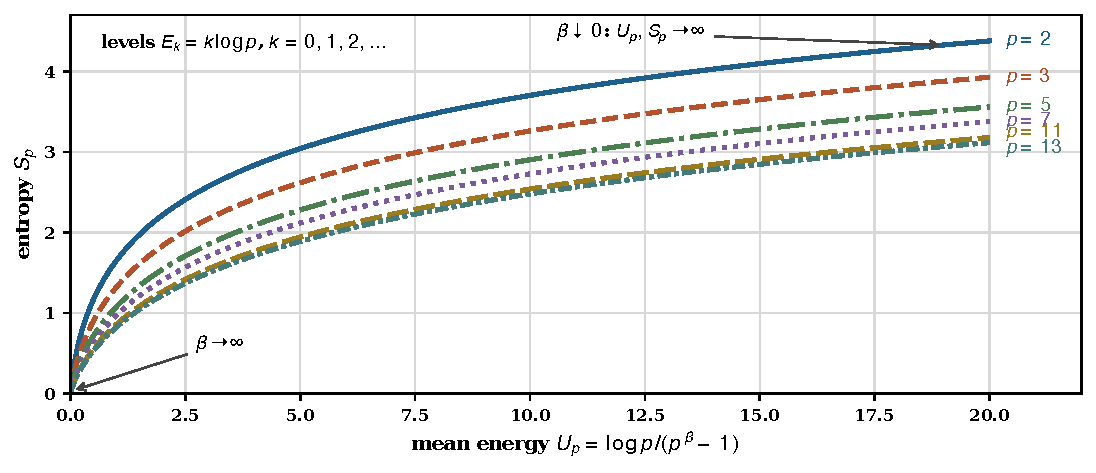
\includegraphics[width=0.96\textwidth]{figures/prime-mode-entropy-energy-curves.pdf}
  \caption{Entropy--energy curves for the first six prime modes
  \(p=2,3,5,7,11,13\), each with levels \(E_k=k\log p\).  The curves are
  distinct in physical energy \(U_p\), but coincide after the horizontal
  rescaling \(U_p\mapsto U_p/\log p\).  Their canonical domain is
  \(\beta>0\); negative temperatures do not define Gibbs states.}
  \label{fig:prime-mode-entropy-energy}
\end{figure}

For the normalized Gibbs law, in units with \(k_B=1\), the mean energy and
entropy are
\[
  U(\beta)=-\frac{d}{d\beta}\log\zeta(\beta),
  \qquad
  S(\beta)=\log\zeta(\beta)+\beta U(\beta).
\]
Figure~\ref{fig:zeta-entropy-energy} plots this parametric entropy--energy
curve.  It has only the branch \(\beta>1\): as \(\beta\to\infty\), both
\(U\) and \(S\) tend to zero, while both diverge as \(\beta\downarrow1\).

\begin{figure}[ht]
  \centering
  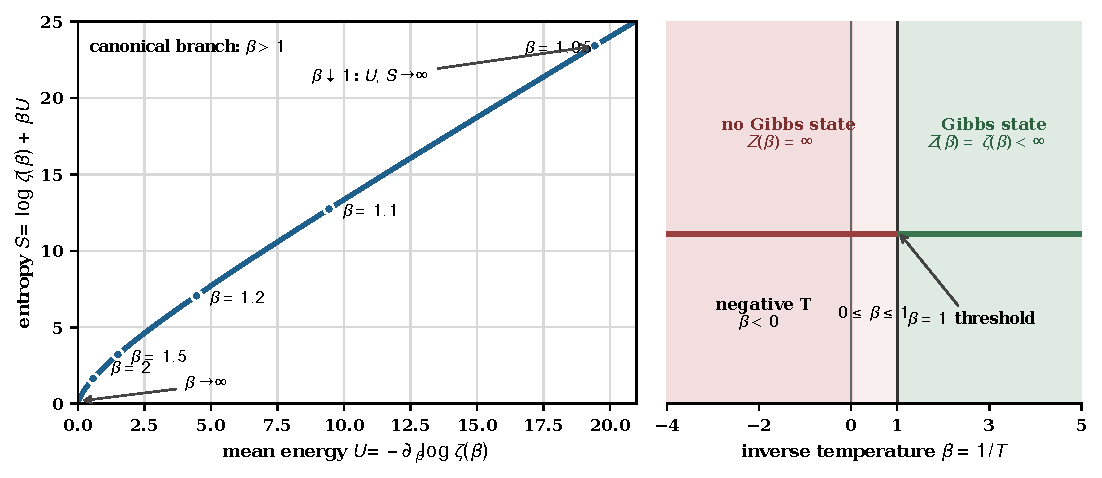
\includegraphics[width=0.98\textwidth]{figures/zeta-entropy-energy.pdf}
  \caption{The canonical entropy--energy curve of the zeta Gibbs system and
  its inverse-temperature domain.  Since the spectrum \(E_n=\log n\) is
  unbounded above, \(\sum_n e^{-\beta E_n}\) diverges for every
  \(\beta\le1\).  Thus the model has no normalized negative-temperature
  branch (\(\beta<0\)); analytic continuation of \(\zeta\) does not supply
  one.}
  \label{fig:zeta-entropy-energy}
\end{figure}

If the exchange-profile formula is applied formally to two individual prime
modes, then
\begin{equation}
  C_{\rm prof}(\operatorname{Atom}(p)\to\operatorname{Atom}(q))
  =\inf_{\beta>0}
  \frac{-\log(1-p^{-\beta})}{-\log(1-q^{-\beta})}
  =
  \begin{cases}
    1,&p\le q,\\
    0,&p>q.
  \end{cases}
  \label{eq:prime-atom-rate}
\end{equation}
Indeed, for \(p<q\) the ratio is at least one and tends to one as
\(\beta\downarrow0\); for \(p>q\) it tends to zero as
\(\beta\to\infty\).  This degenerate answer is informative: over the full
temperature range, unequal infinite ladders do not have matching low- and
high-temperature asymptotics.  A nontrivial comparison needs a temperature
window, a work offset, or a different operational model.  Equation
\eqref{eq:prime-atom-rate} is therefore a profile calculation, not a new
coding theorem for primes.

\clearpage
\subsection{Complex temperature and zeros}

For \(\beta>1\), normalize the Gibbs law
\[
  \Pr_\beta(N=n)=\frac{n^{-\beta}}{\zeta(\beta)}.
\]
Then
\begin{equation}
  \frac{\zeta(\beta+it)}{\zeta(\beta)}
  =\mathbb E_\beta\!\left[e^{-it\log N}\right]
  \label{eq:zeta-characteristic}
\end{equation}
is the characteristic function of the random log-energy.  A zero in this
half-plane would be exact destructive phase cancellation, but the Euler
product proves that no such zero exists.

The nontrivial zeros lie in \(0<\Re s<1\), outside the normalizable Gibbs
regime of \eqref{eq:zeta-partition}.  Analytic continuation assigns values
there, but no positive probability measure \(n^{-1/2}/\zeta(1/2)\) exists.
Consequently
\[
  \rho=\frac12+i\gamma
\]
should not presently be called a literal complex energy level.  A safer
statement is that \(\gamma\) is a logarithmic Mellin frequency: terms such as
\(x^\rho=x^{1/2}e^{i\gamma\log x}\) oscillate in log scale in explicit
formulas.

The quantum-chaos analogy reverses the roles.  It seeks an unknown Hermitian
Hamiltonian whose eigenvalues are the ordinates \(\gamma\), while the prime
powers \(p^k\) contribute periodic-orbit lengths \(k\log p\).  Berry and
Keating's \(H=xp\) program is a prominent version of this analogy
\cite{berry-keating}.  It does not currently identify a zero with a quantum
composition of the independent prime modes in \eqref{eq:zeta-partition}.

\subsection{What the completion adds}

The completed function
\[
  \xi(s)=\frac12s(s-1)\pi^{-s/2}\Gamma(s/2)\zeta(s)
\]
has three conceptually different pieces.
\begin{enumerate}
  \item \(\zeta(s)=\prod_p(1-p^{-s})^{-1}\) is the product of the finite-prime
  local factors.
  \item \(\pi^{-s/2}\Gamma(s/2)\) is the archimedean local factor, obtained
  as the Mellin transform of a Gaussian.
  \item \(s(s-1)/2\) cancels the poles at \(0\) and \(1\), producing an
  entire function.
\end{enumerate}
If
\[
  \theta(t)=\sum_{n\in\mathbb Z}e^{-\pi n^2t},
\]
then for \(\Re s>1\)
\[
  \int_0^\infty(\theta(t)-1)t^{s/2}\,\frac{dt}{t}
  =2\pi^{-s/2}\Gamma(s/2)\zeta(s).
\]
Poisson summation gives \(\theta(t)=t^{-1/2}\theta(1/t)\), and splitting the
integral at \(t=1\) yields analytic continuation and the reflection
\[
  \xi(s)=\xi(1-s).
\]
In Tate's adelic formulation, the finite and archimedean factors are local
Mellin transforms and the functional equation is global Fourier duality
\cite{tate-thesis}.  For the Gibbs analogy, this is the main lesson of the
completion: the global object is not only a product of positive local
oscillators; it is completed by a self-dual archimedean mode and a scale
reflection.

\section{The Weil matrix \texorpdfstring{\(E\)}{E} and the rate matrix
\texorpdfstring{\(M\)}{M}}
\label{sec:weil}

For an admissible test profile \(g\) with Mellin transform \(\widehat g\), the
Weil quadratic form may be written schematically as
\[
  Q_W(g)=\sum_\rho
  \widehat g(\rho)
  \overline{\widehat g(1-\overline\rho)},
\]
with the standard symmetric convergence.  Polarization gives
\(B_W(g,h)\), and a finite family gives the Hermitian matrix
\[
  E_{ij}=B_W(g_i,g_j).
\]
Weil's explicit-formula criterion says that positivity for every admissible
family is equivalent to the Riemann hypothesis
\cite{weil-explicit}.  Under RH, \(1-\overline\rho=\rho\), so \(E\) becomes a
Gram matrix of the sampled Mellin transforms.

This matrix and the operational exchange matrix have different definitions:
\begin{center}
\begin{tabular}{@{}p{0.24\textwidth}p{0.34\textwidth}p{0.34\textwidth}@{}}
\toprule
 & rate matrix \(M\) & Weil matrix \(E\)\\
\midrule
input & maps and allowed processors & admissible Mellin test profiles\\
direction & directed & Hermitian\\
composition law & \(M_{ij}M_{jk}\le M_{ik}\) & sesquilinear polarization\\
positivity notion & no profitable cycle & positive semidefinite quadratic form\\
arithmetic data & implementation counts & primes, gamma factor, and zeros\\
known bridge & none in this paper & none in this paper\\
\bottomrule
\end{tabular}
\end{center}

One exploratory construction multiplies a map profile \(\mathcal Z_i(s)\) by
a log-Gaussian Mellin window and samples the first \(N\) known critical-line
zeros.  With \(\sigma=1/20\), omitting a common positive factor, the real
matrix is
\[
  E^{(N)}_{ij}
  =2\sum_{n=1}^N e^{-\gamma_n^2/400}
  \operatorname{Re}\!\left(
    \overline{\mathcal Z_i(\rho_n)}\mathcal Z_j(\rho_n)
  \right).
\]
For zeros already sampled on the critical line this is visibly a Gram matrix,
so its positive semidefiniteness is automatic.  For \(N=100\), the observed
ranks are:
\begin{center}
\begin{tabular}{@{}lrr@{}}
\toprule
family & nodes & rank\\
\midrule
quadratic ternary forms over \(\F_3\) & 5 & 5\\
quadratic homogeneous \(\F_3^2\to\F_3^2\) & 7 & 6\\
displayed quadratic representatives over \(\Q_3\) & 8 & 5\\
displayed quadratic representatives over \(\Q_2\) & 12 & 5\\
\bottomrule
\end{tabular}
\end{center}
The rank losses come from exact profile identities or repeated local zeta
profiles.  They say nothing yet about affine conversion.  In particular,
positive semidefiniteness of these finite-height Gram matrices is not evidence
that no-arbitrage implies Weil positivity, and it is not an independent test
of RH.

To connect \(M\) and \(E\), one would need at least:
\begin{enumerate}
  \item a canonical assignment from polynomial-map resources to admissible
  adelic test profiles;
  \item compatibility of that assignment with processor composition and
  Cartesian powers;
  \item a theorem translating operational inequalities into the
  sesquilinear explicit formula, or conversely.
\end{enumerate}
No such construction is presently known here.

\section{What is classical, what is new, and what is open}
\label{sec:novelty}

The main contribution is a new angle and a reproducible synthesis, not a claim
to have rediscovered quadratic-form theory.  The following ledger states the
current novelty boundary.

\begin{center}
\begin{tabular}{@{}p{0.26\textwidth}p{0.29\textwidth}p{0.37\textwidth}@{}}
\toprule
topic & prior status & contribution and claim level\\
\midrule
left--right equivalence & classical in singularity and orbit theory & use
the same processor equation simultaneously for equivalence, exact singular
reachability, and block exchange\\[2pt]
quadratic normal forms & classical Witt, discriminant, radical, and Arf theory
& a uniform resource-oriented derivation of the nodes and arrow direction
over finite, real, complex, and local fields\\[2pt]
finite-field quadratic counts & consequences of classical orbit--stabilizer
calculations & closed formulas and a reproducible atlas of class-sized Hasse
diagrams for all odd \(q\), all even \(q\ge4\), and the exceptional \(q=2\)
case; the exact compilation appears to be new, but not the ingredients\\[2pt]
homogeneous and cubic cases & instances belong to invariant theory and
finite computation & candidate new computational datasets: the \(\F_3\)
five-, seven-, fifty-, twenty-six-, and nineteen-class diagrams, and the
\(110\)-class generated preorder over \(\F_8\)\\[2pt]
asymptotic rates & resource theories and asymptotic spectra are classical;
the signature formula is proved in the companion paper & attach the solved
signature rate to polynomial-map orbit nodes while explicitly separating it
from the affine operational rate\\[2pt]
cycle return & cycle means and max--plus algorithms are classical & apply them
to map-class exchange matrices as round-trip-loss and observer-resolution
diagnostics\\[2pt]
zeta as partition function & Euler product and Bost--Connes are classical &
place the prime-mode Gibbs picture next to map profiles and show exactly where
the analogy ceases to be an ordinary Gibbs system\\[2pt]
RH and Weil positivity & classical Weil criterion & no new RH claim; the
missing \(M\)-to-\(E\) bridge is formulated as an open problem\\
\bottomrule
\end{tabular}
\end{center}

Three items are the strongest candidates for genuinely new results after a
full literature review:
\begin{enumerate}
  \item the explicit all-\(q\) affine-processor Hasse atlas for
  degree-at-most-two maps \(\F_q^2\to\F_q\), with orbit sizes at every node;
  \item the exhaustive homogeneous and cubic finite-field datasets and their
  verification programs;
  \item the combined study of the exact degeneration poset, the solved
  fiber-signature exchange observer, and the max--times cycle losses on the
  same named classes.
\end{enumerate}
These should be advertised as new computations and organization unless a
prior source is found.  The no-arbitrage proof itself is elementary and should
not be sold as a deep new theorem; its value is that it places a precise
constraint on every rate matrix generated by the framework.

\section{Open problems}

\begin{question}[Affine coding theorem]
Can \(\caff(g\to f)\) be characterized by a complete family of algebraic or
analytic monotones, analogous to the partition functions that solve the
finite-signature theory?
\end{question}

\begin{question}[The seven \(2\)-adic anisotropic classes]
Are distinct anisotropic binary forms over \(\Q_2\) asymptotically
interconvertible at a rate strictly greater than \(1/2\)?  Does any pair have
rate one without a finite rate-one conversion?
\end{question}

\begin{question}[Cycle separation]
For which processor categories does a uniform gap
\(r(\mathcal C)\le1-\varepsilon\) over all nontrivial cycles characterize an
asymptotic separation of equivalence classes?  When does a cycle mean of one
imply asymptotic reversibility rather than merely a coarse observer?
\end{question}

\begin{question}[Functorial zeta profiles]
Is there a lattice-independent or adelic profile assignment that is monotone
under affine implementation, multiplicative under Cartesian products, and
rich enough to bound or determine \(\caff\)?
\end{question}

\begin{question}[The \(M\)-to-\(E\) bridge]
Can a natural completion of polynomial-map resources produce admissible Weil
test functions in a way that turns no-arbitrage or conversion monotonicity
into positivity of a Hermitian form?  A successful answer must explain why a
directed max--times matrix should control a sesquilinear matrix; superficial
entrywise transformations are insufficient.
\end{question}

\section{Conclusion}

The equation \(f=h_{\rm out}\circ g\circ h_{\rm in}\) is deliberately
small.  With invertible affine processors it gives classical equivalence
classes.  With singular affine processors it gives a degeneration preorder
and Hasse diagrams.  With Cartesian powers it gives exchange rates, directed
triangle inequalities, and no-arbitrage cycle bounds.  With the fiber
signature observer it gives partition functions and Gibbs curves already
solved in the companion paper.

Quadratic maps show the benefit of the framework because the answer is
recognizable: rank, radical, isotropy, discriminant, and the Arf/trace
invariant reappear as resource monotones and branching rules.  The same
language continues from finite fields to real, complex, and \(p\)-adic
analytic maps, and from scalar quadratics to homogeneous tensors and cubics.

The number-theoretic continuation is promising but incomplete.  The Euler
product really is a joint partition function of prime occupation modes for
\(\Re s>1\); the completed zeta function really is assembled from finite and
archimedean local factors and Fourier--Mellin duality.  But the nontrivial
zeros are not ordinary Gibbs energy levels, and the operational matrix \(M\)
is not the Weil matrix \(E\).  The present contribution is to make the common
language precise enough that a future bridge, if it exists, will have a clear
mathematical statement.

\appendix
\section{A visual atlas over finite fields}
\label{sec:visual-atlas}

The formulas in Section~\ref{sec:quadratic-normal-forms} say that all odd
finite fields share one six-node shape, while all even fields of order at
least four share one seven-node shape.  The diagrams below retain the shape
and change the orbit sizes.  They are included because the class-size labels
make the orbit formulas concrete, and because the exceptional \(\F_2\)
collapse is easiest to remember visually.

\begin{figure}[p]
  \centering
  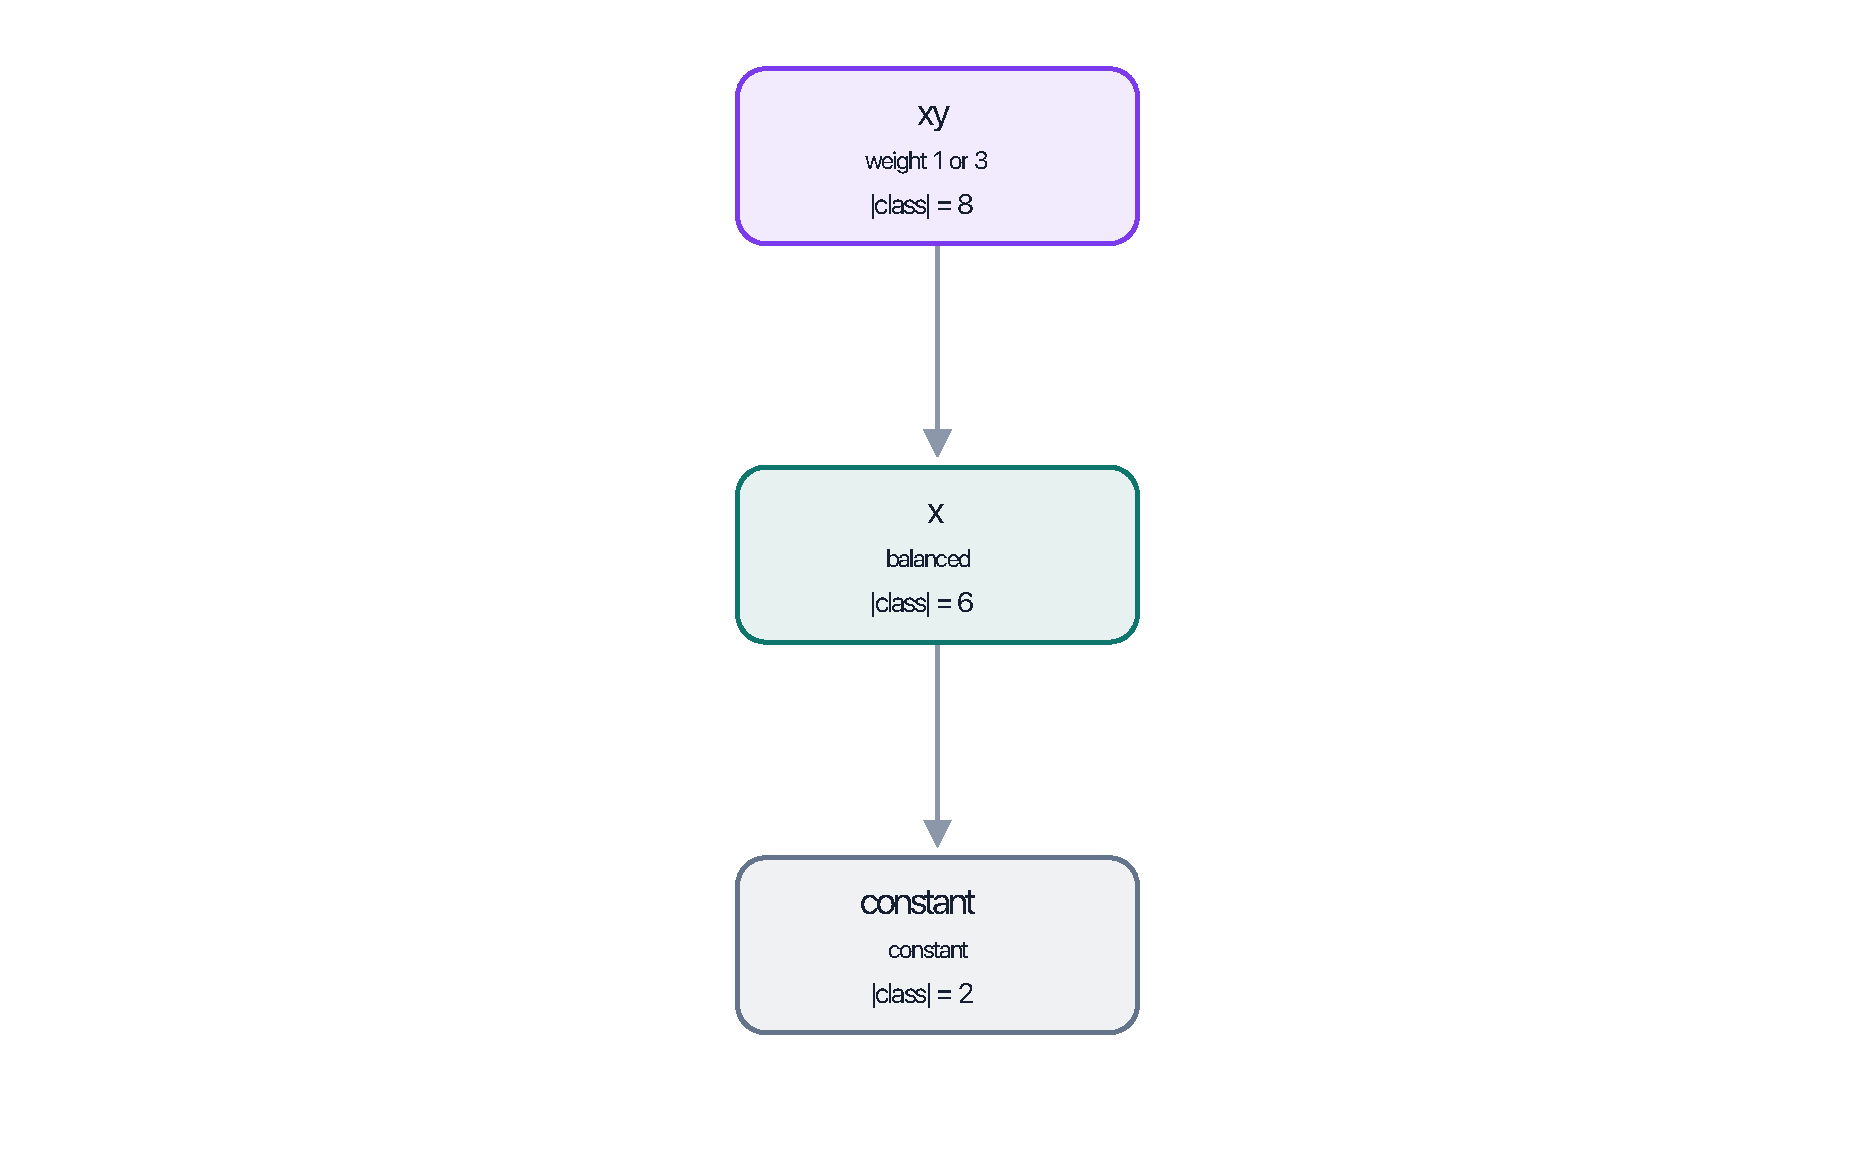
\includegraphics[width=0.62\textwidth,height=0.31\textheight,keepaspectratio]{figures/quadratic-map-poset-q2.pdf}
  \par\medskip
  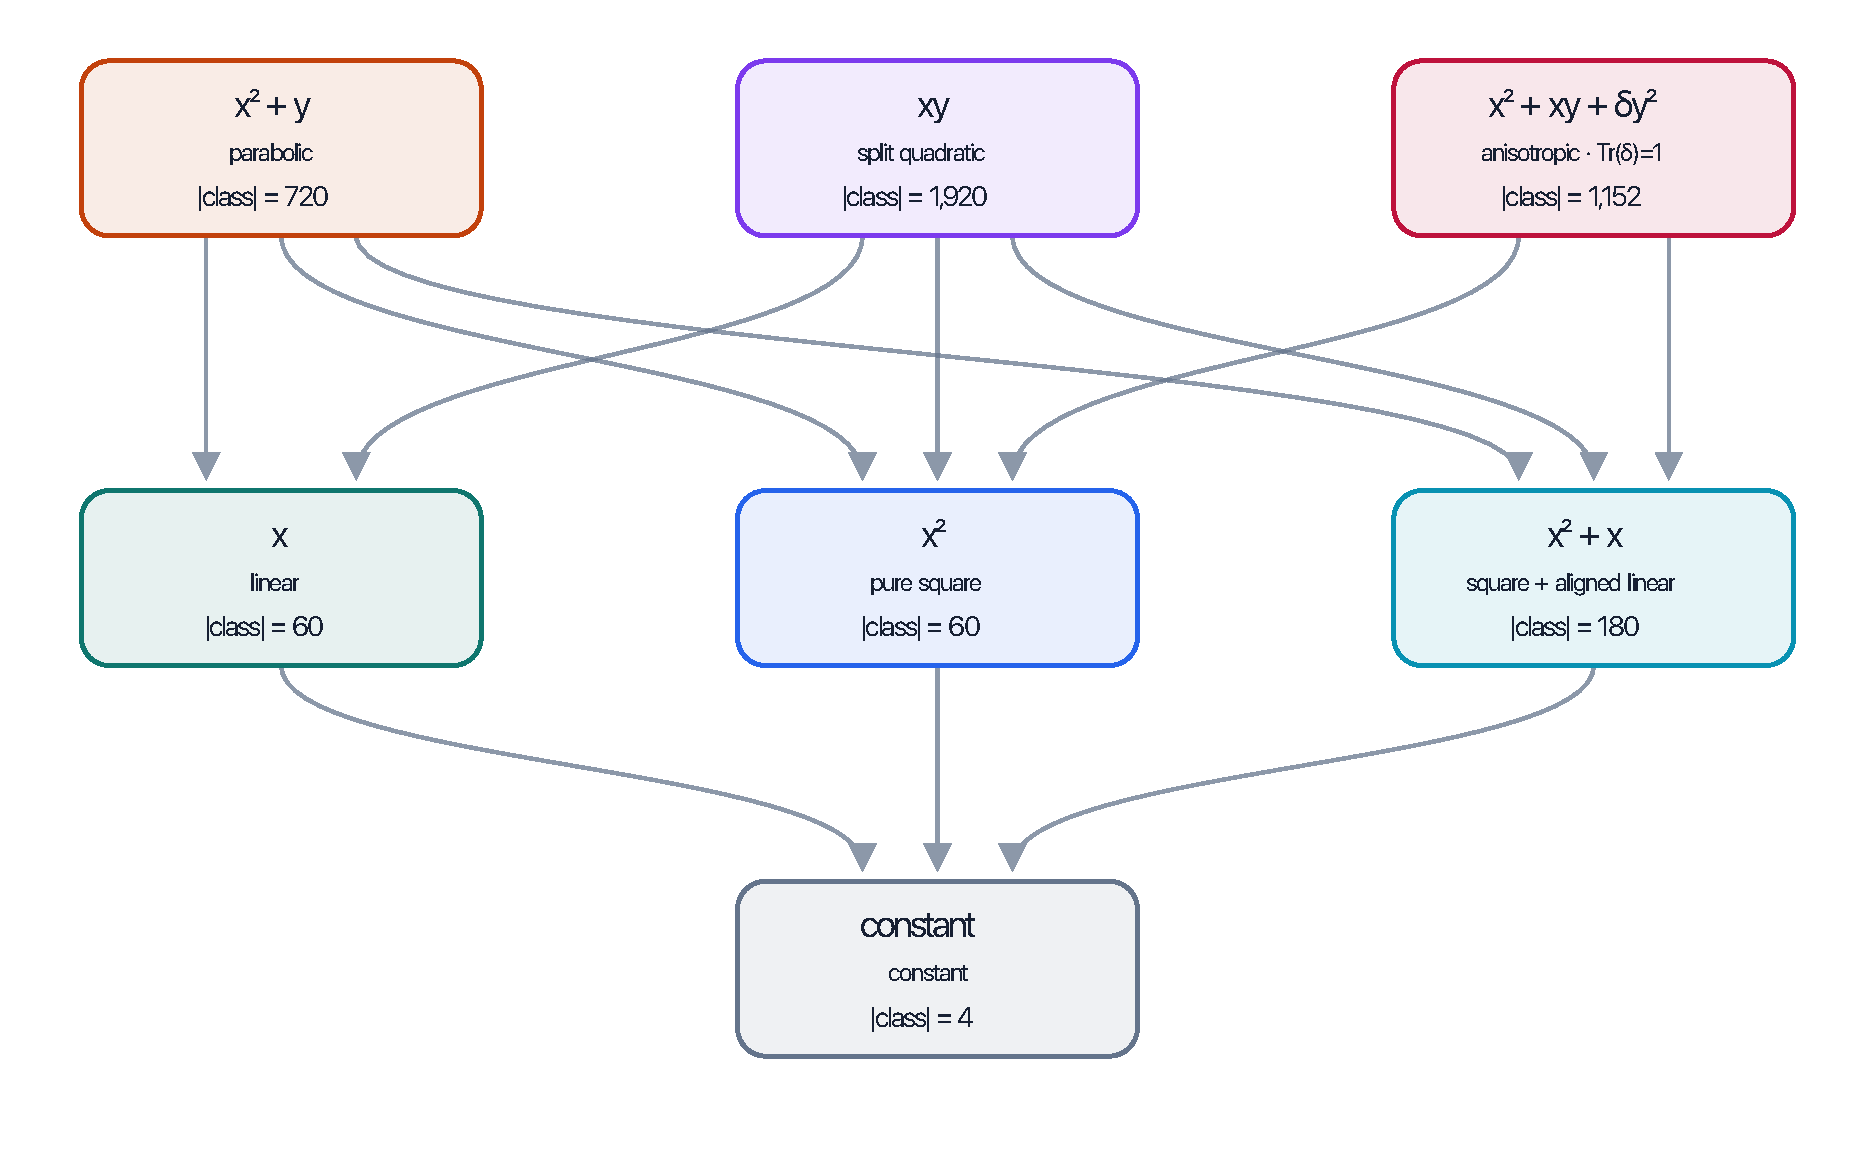
\includegraphics[width=0.62\textwidth,height=0.31\textheight,keepaspectratio]{figures/quadratic-map-poset-q4.pdf}
  \caption{The exceptional three-class, two-cover function poset over
  \(\F_2\), followed by the generic seven-class, eleven-cover poset over
  \(\F_4\).  Both use possibly singular affine processors.}
\end{figure}

\begin{figure}[p]
  \centering
  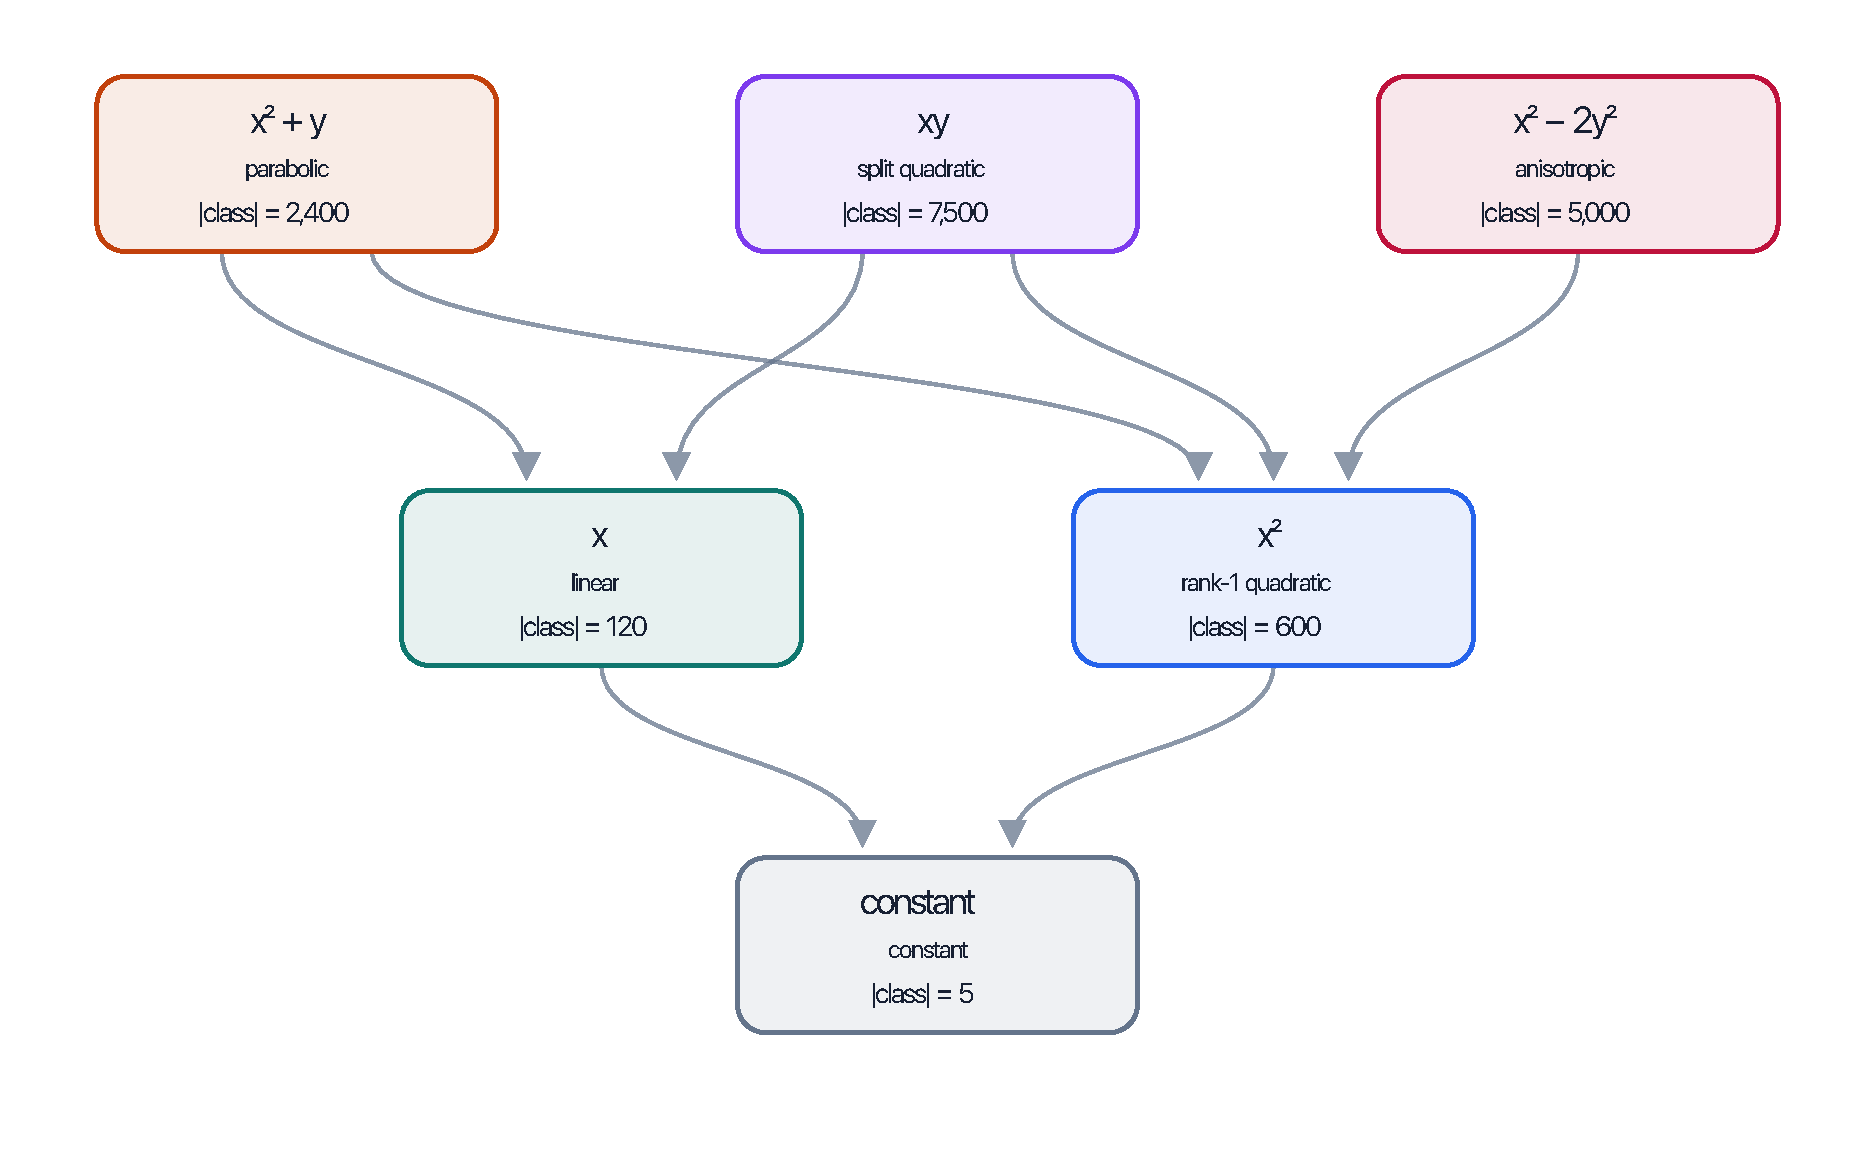
\includegraphics[width=0.62\textwidth,height=0.31\textheight,keepaspectratio]{figures/quadratic-map-poset-q5.pdf}
  \par\medskip
  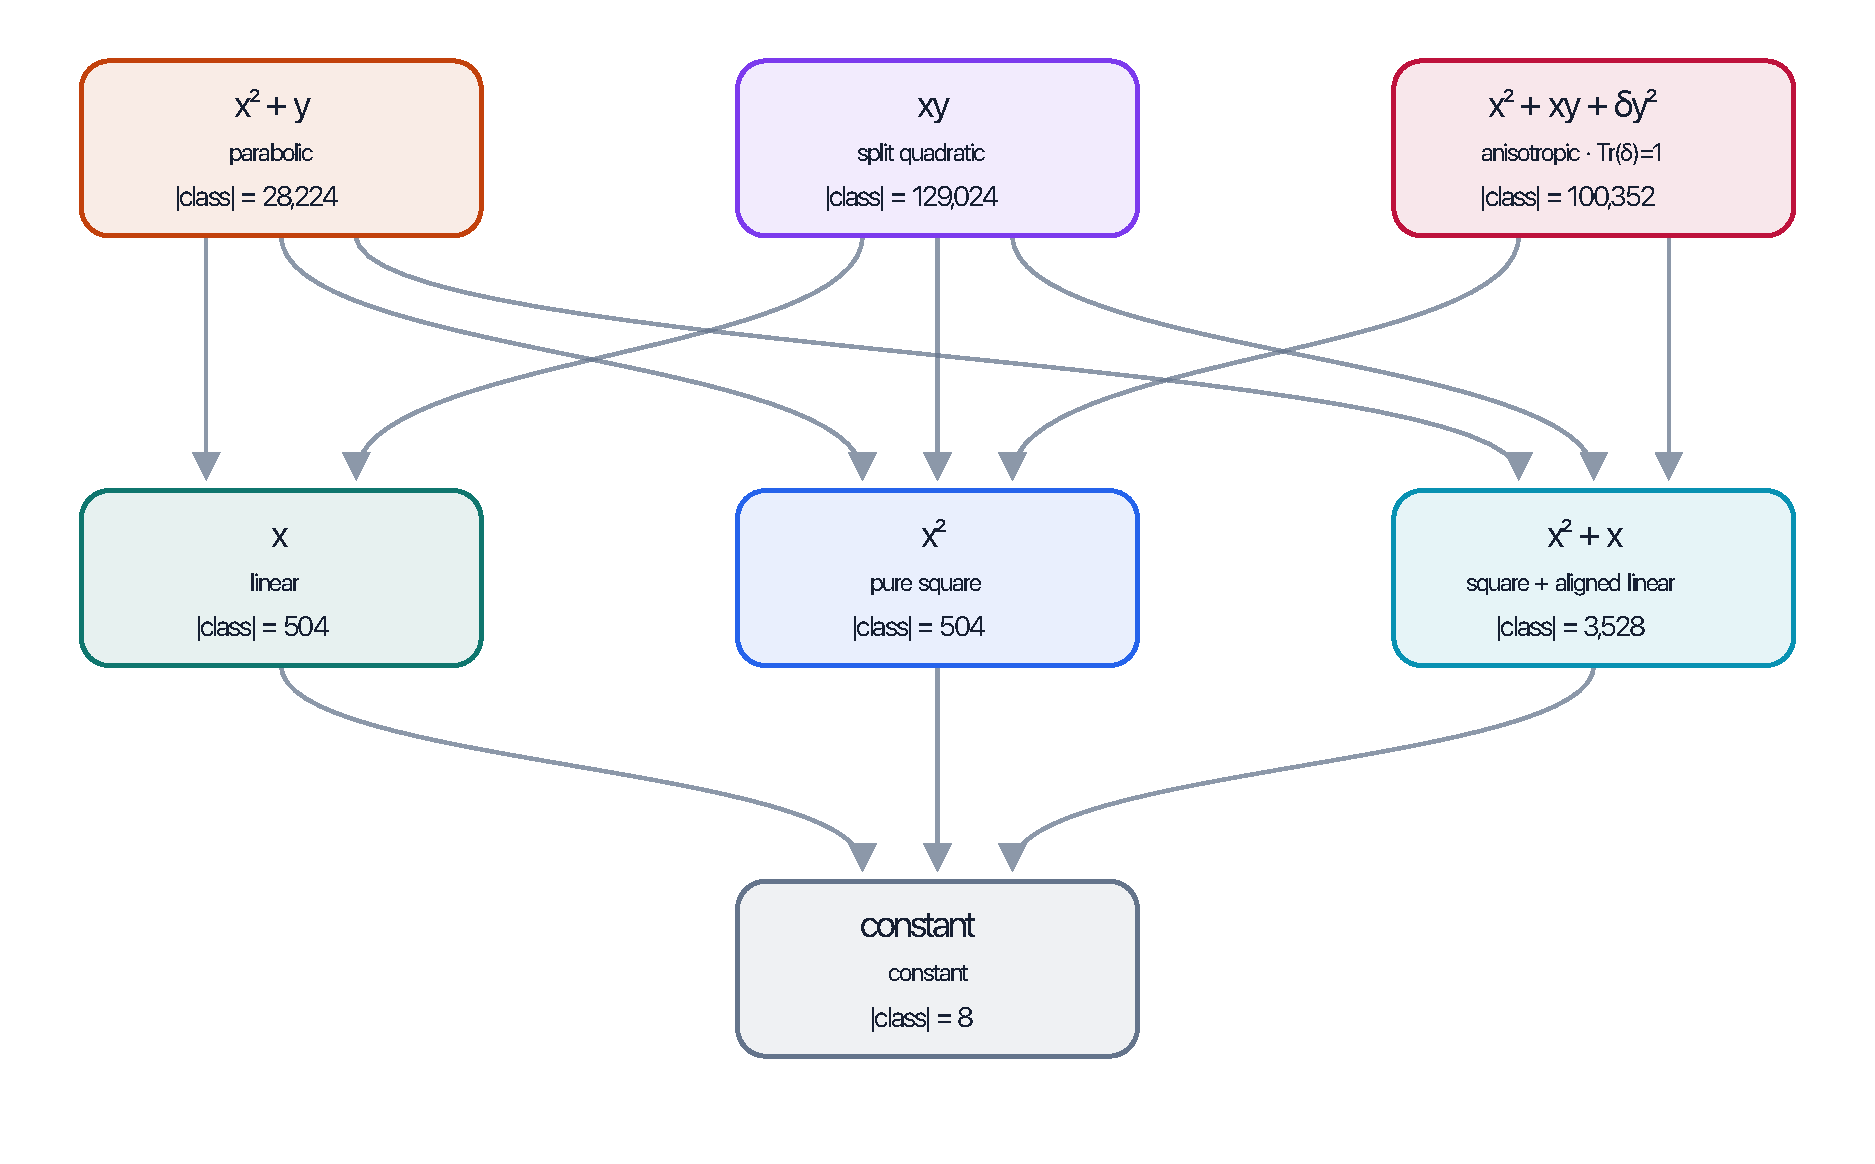
\includegraphics[width=0.62\textwidth,height=0.31\textheight,keepaspectratio]{figures/quadratic-map-poset-q8.pdf}
  \caption{Quadratic maps with singular affine processors over \(\F_5\)
  (six classes, seven covers) and \(\F_8\) (seven classes, eleven covers).
  The field parity changes both the normal forms and the poset shape.}
\end{figure}

\begin{figure}[p]
  \centering
  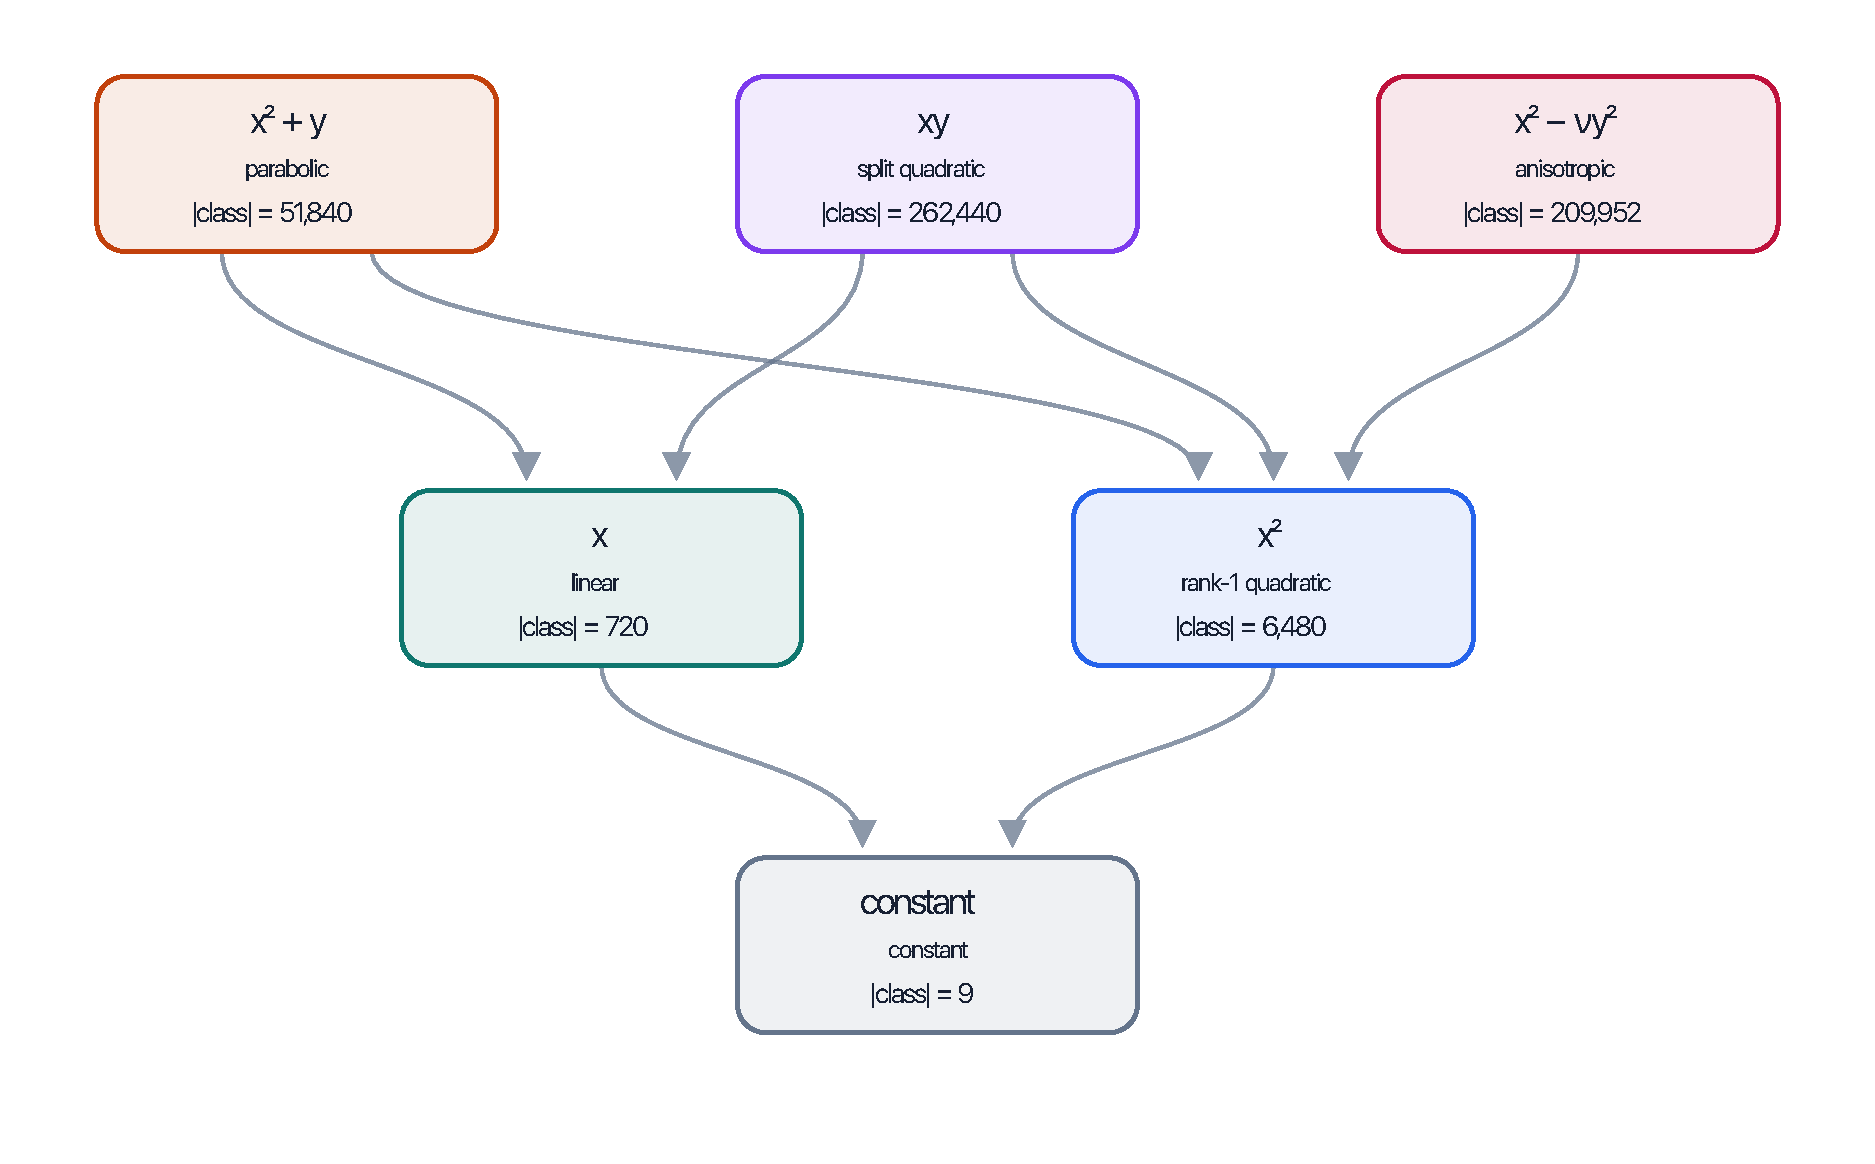
\includegraphics[width=0.78\textwidth,height=0.46\textheight,keepaspectratio]{figures/quadratic-map-poset-q9.pdf}
  \caption{Quadratic maps over \(\F_9\) with singular affine processors:
  six classes and seven covers.  The node labels record the
  field-dependent orbit sizes.}
\end{figure}

\begin{figure}[p]
  \centering
  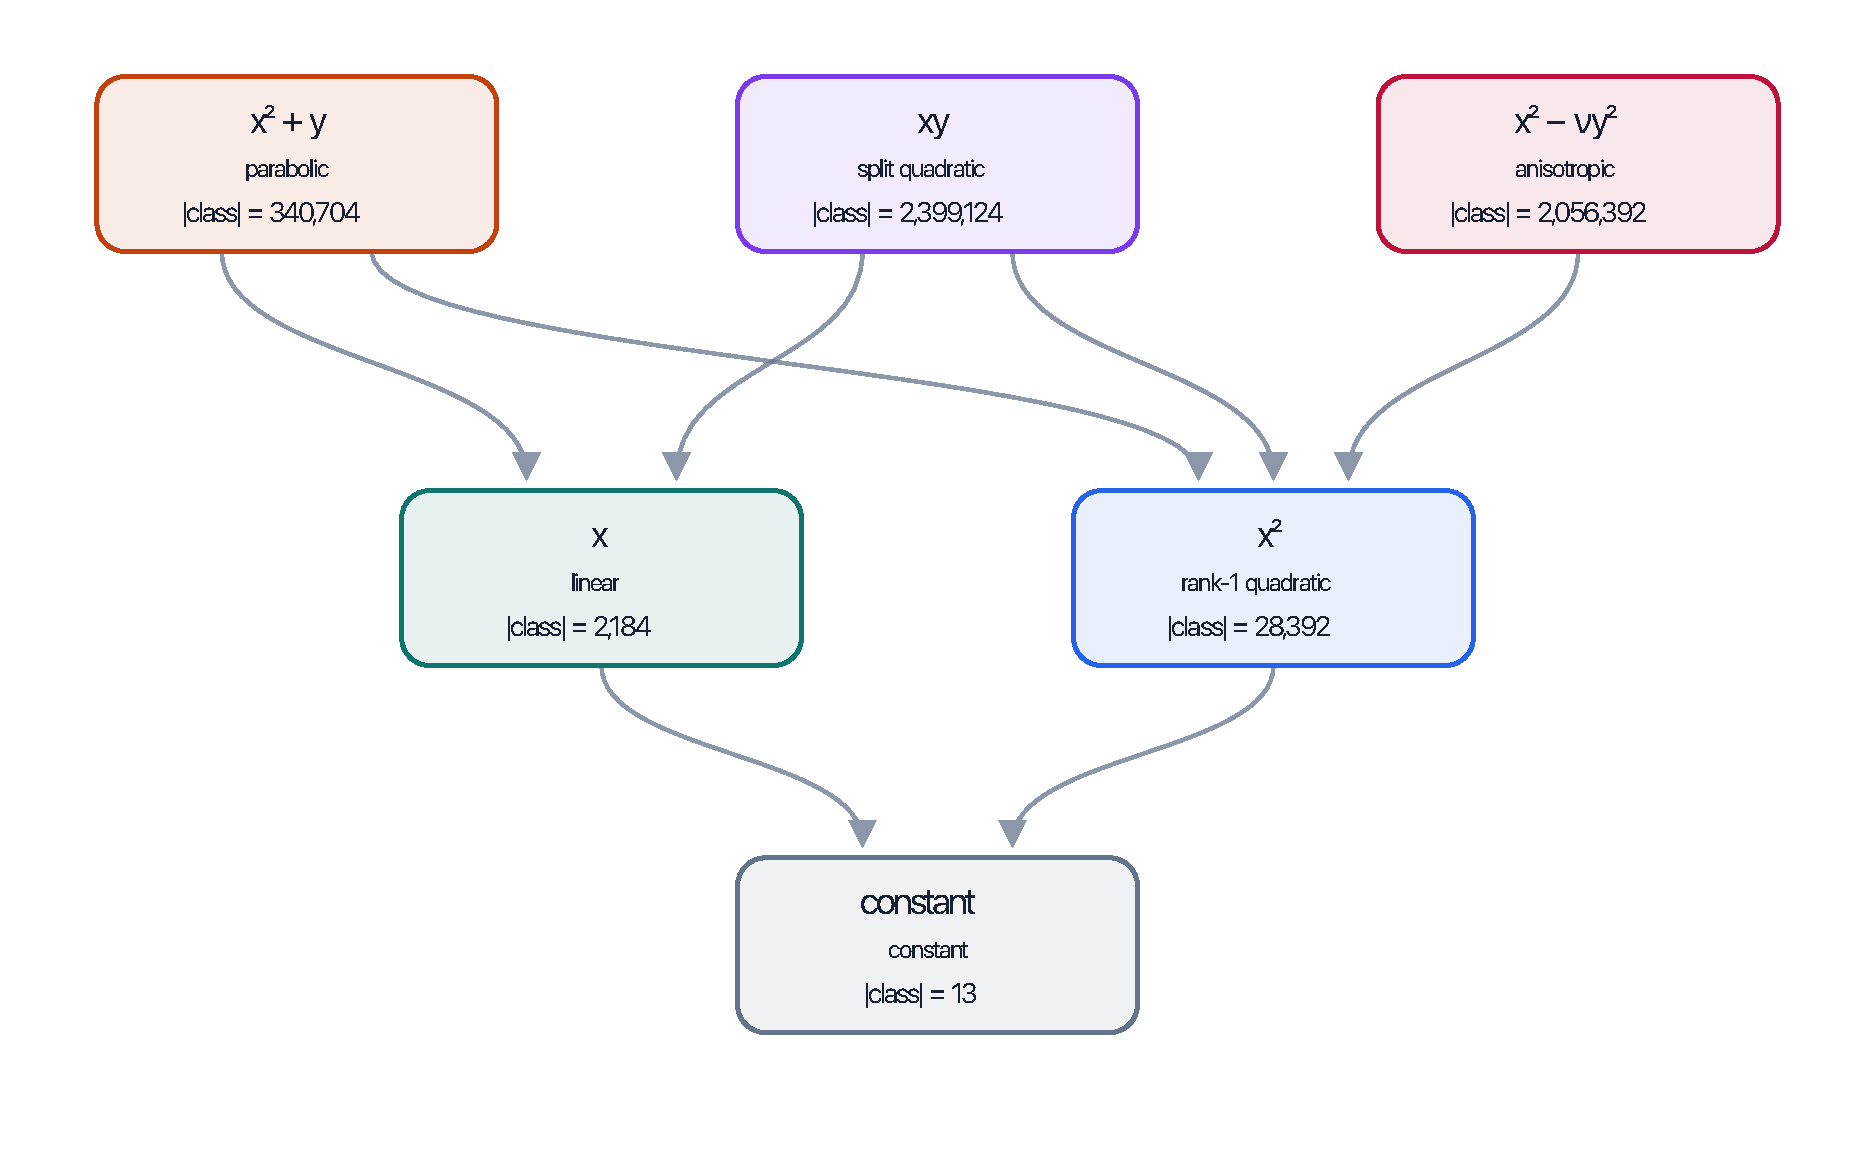
\includegraphics[width=0.62\textwidth,height=0.31\textheight,keepaspectratio]{figures/quadratic-map-poset-q13.pdf}
  \par\medskip
  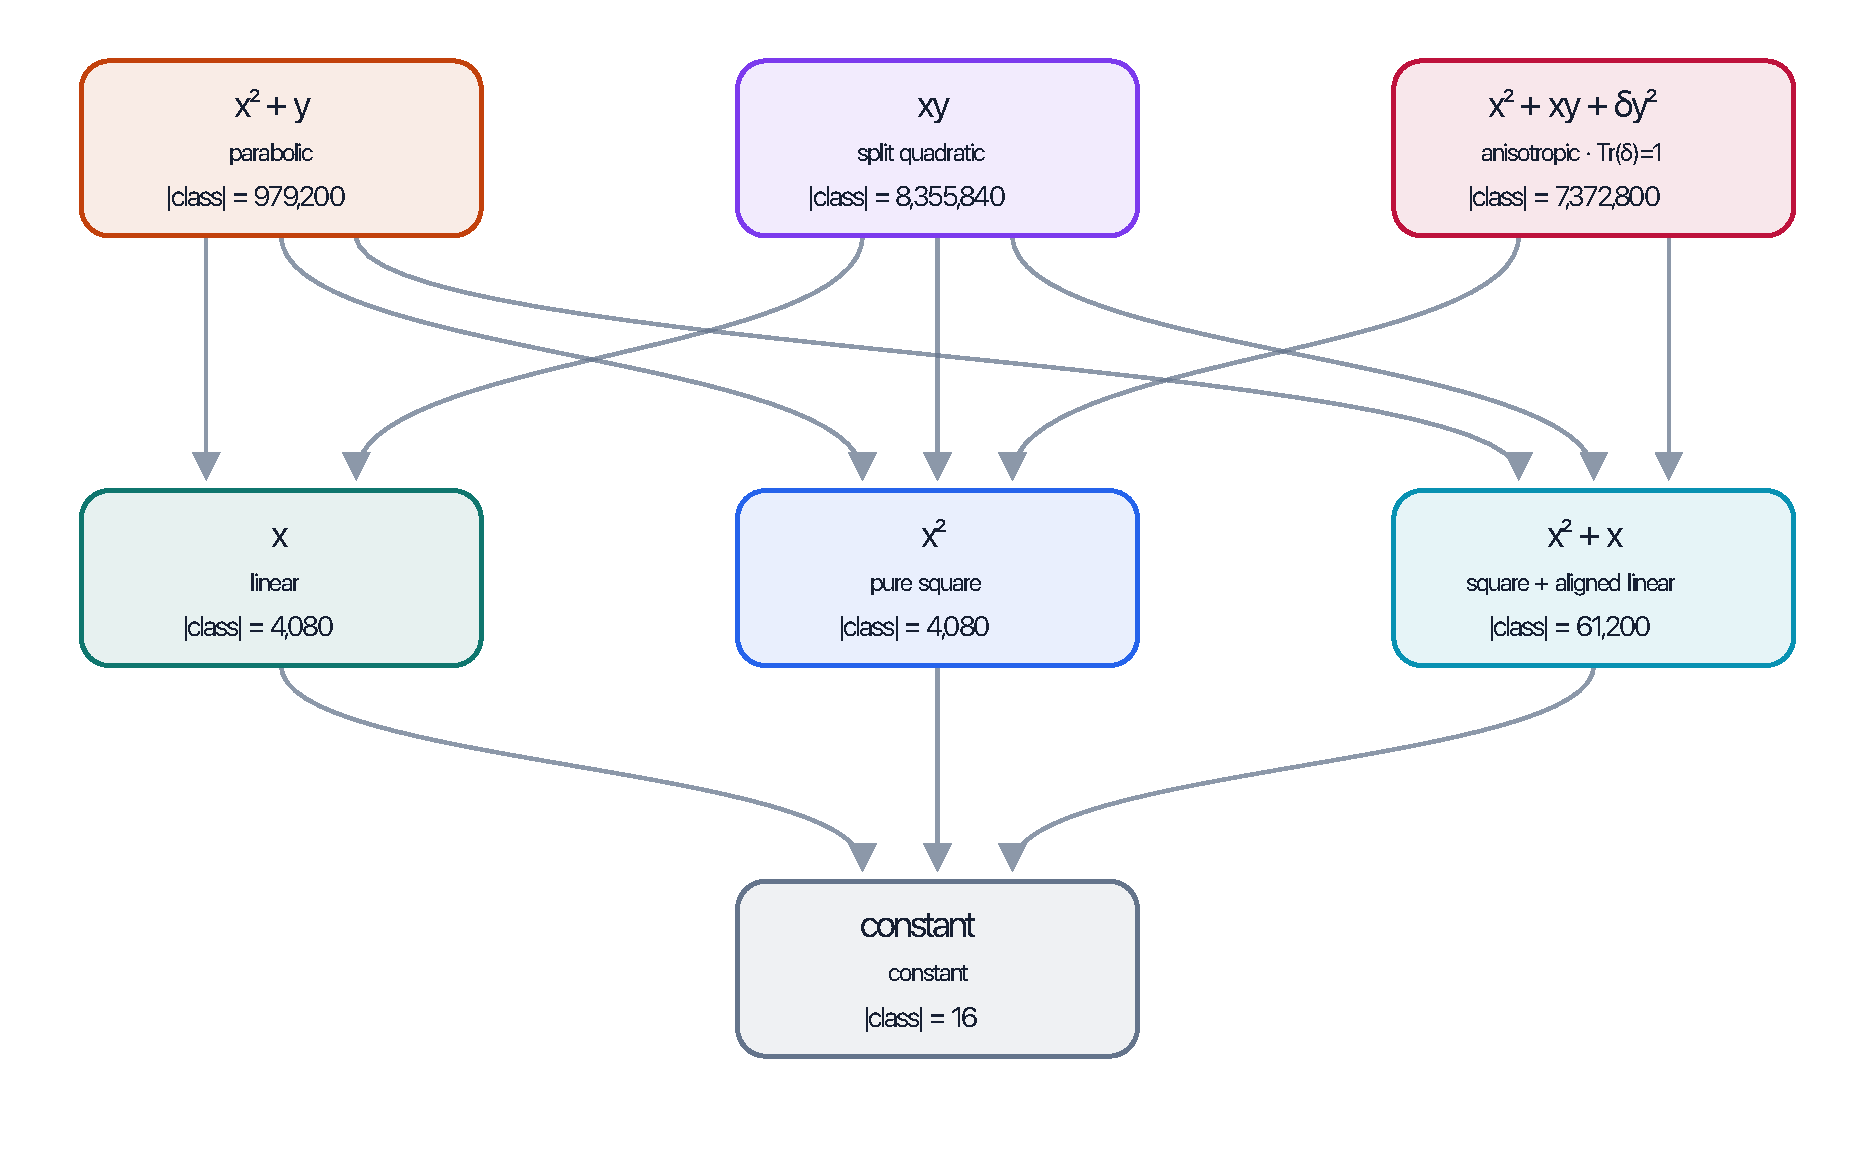
\includegraphics[width=0.62\textwidth,height=0.31\textheight,keepaspectratio]{figures/quadratic-map-poset-q16.pdf}
  \caption{Quadratic maps with singular affine processors over \(\F_{13}\)
  (six classes, seven covers) and \(\F_{16}\) (seven classes, eleven covers).}
\end{figure}

\begin{figure}[p]
  \centering
  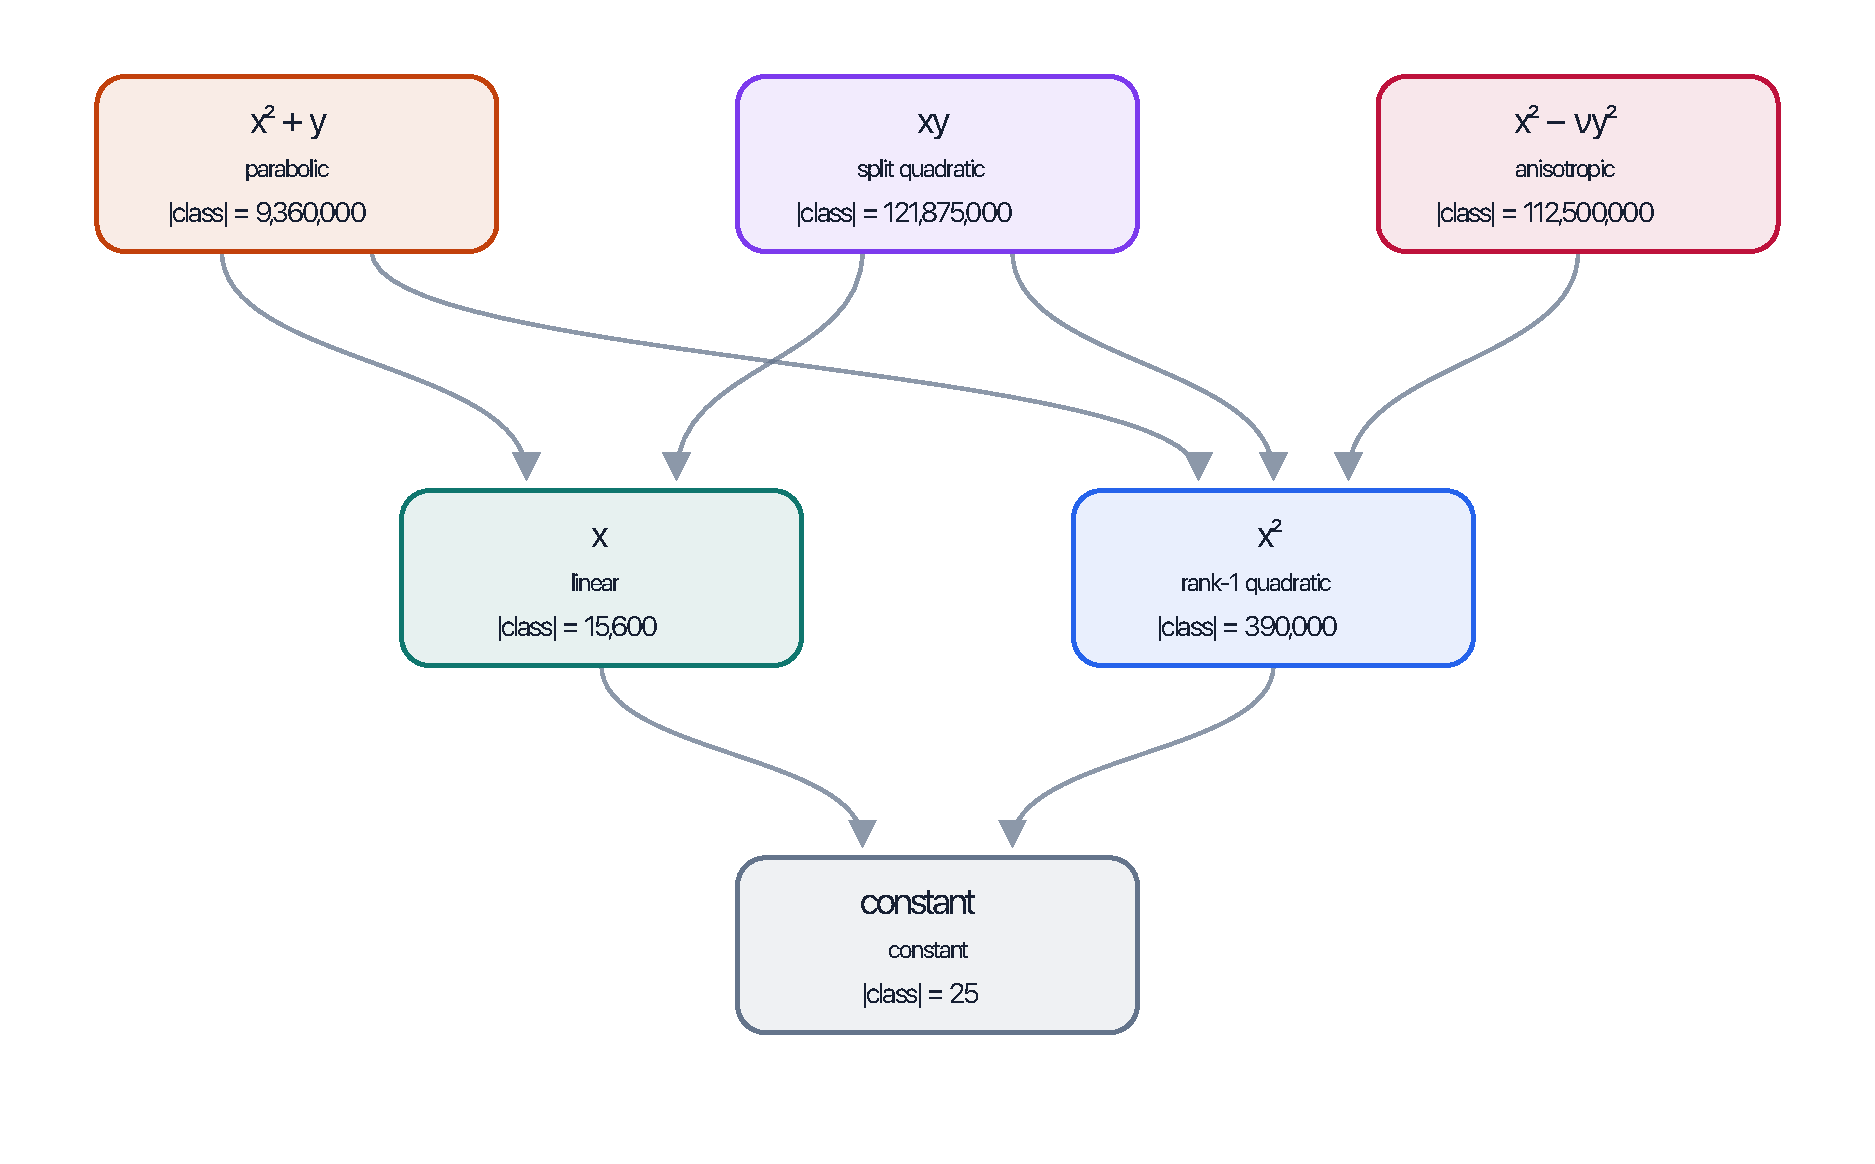
\includegraphics[width=0.76\textwidth]{figures/quadratic-map-poset-q25.pdf}
  \caption{The odd-field diagram over \(\F_{25}\), containing
  \(25^6=244{,}140{,}625\) coefficient vectors in six affine classes and
  seven covers; singular affine processors define the order.}
\end{figure}

\section{Two cubic processor choices}

The next pair shows why the processor class is part of the theorem.  The
underlying universe is the same set of \(6{,}561\) cubic polynomial functions
\(\F_3^2\to\F_3\).  Affine input processors retain fourteen classes.  The
preorder generated by quadratic input processors collapses them to three.

\clearpage
\begin{landscape}
  \begin{figure}[p]
    \centering
    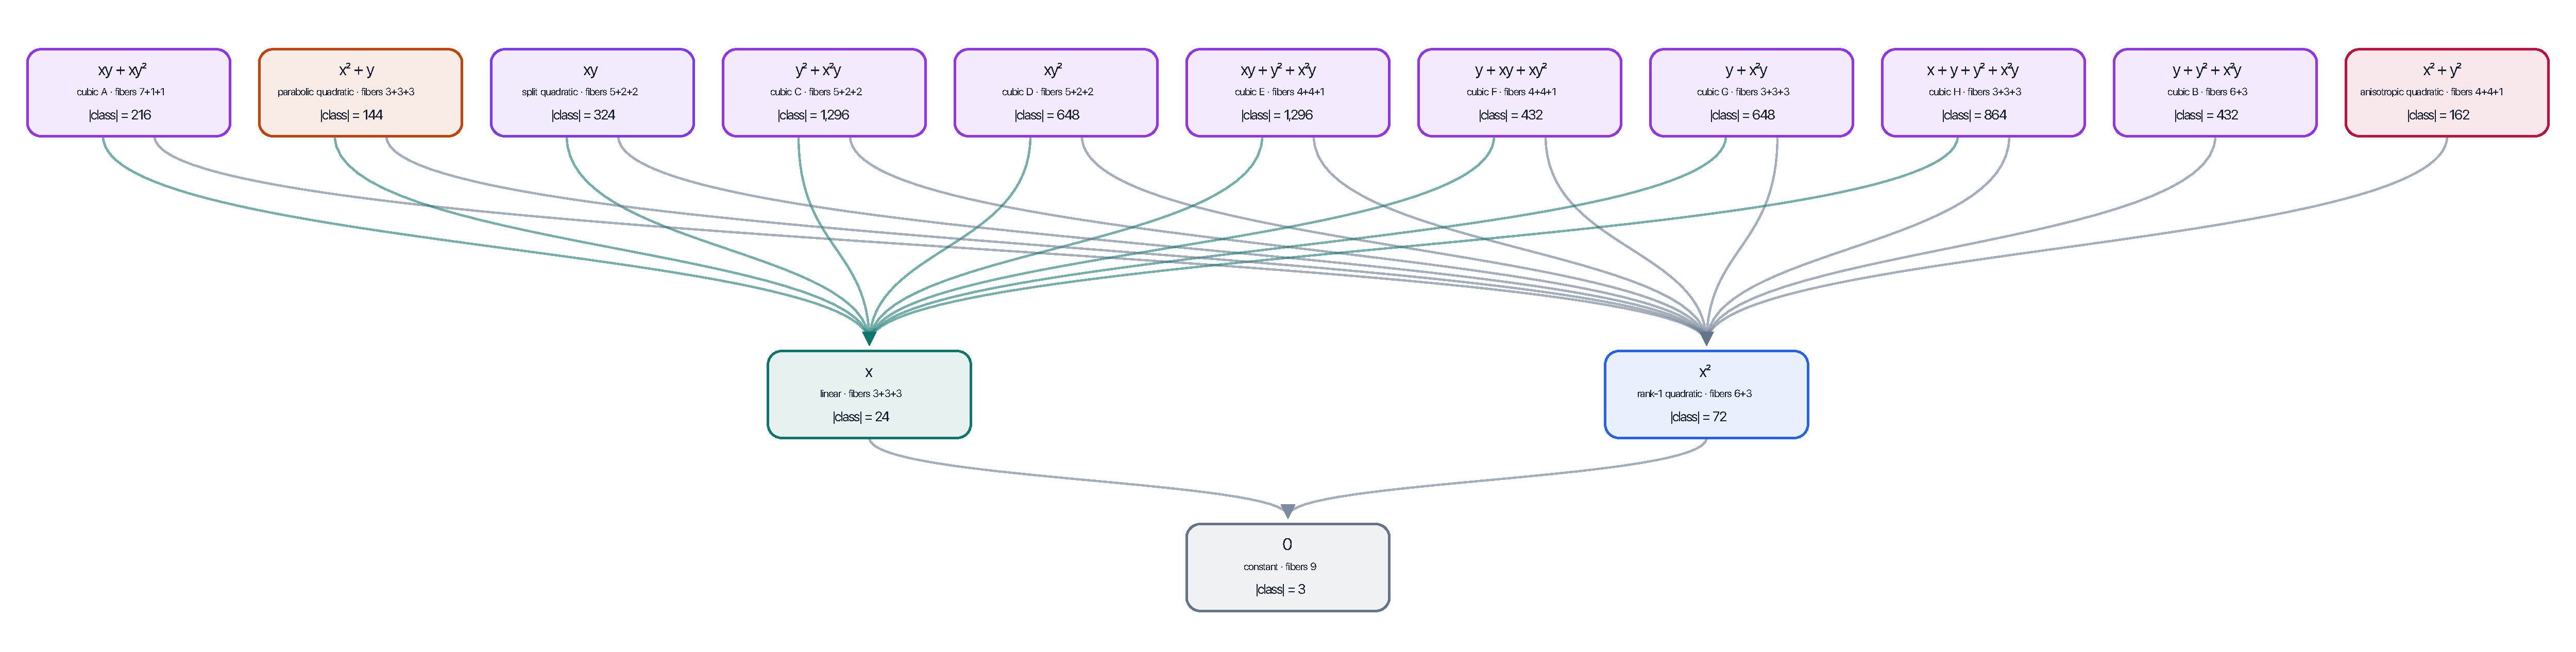
\includegraphics[width=0.96\linewidth,height=0.72\textheight,keepaspectratio]{figures/cubic-map-poset-q3-linear-input.pdf}
    \caption{Cubic functions over \(\F_3\) with affine input and output
    processors: fourteen equivalence classes and twenty-two Hasse covers.}
  \end{figure}
\end{landscape}

\begin{figure}[p]
  \centering
  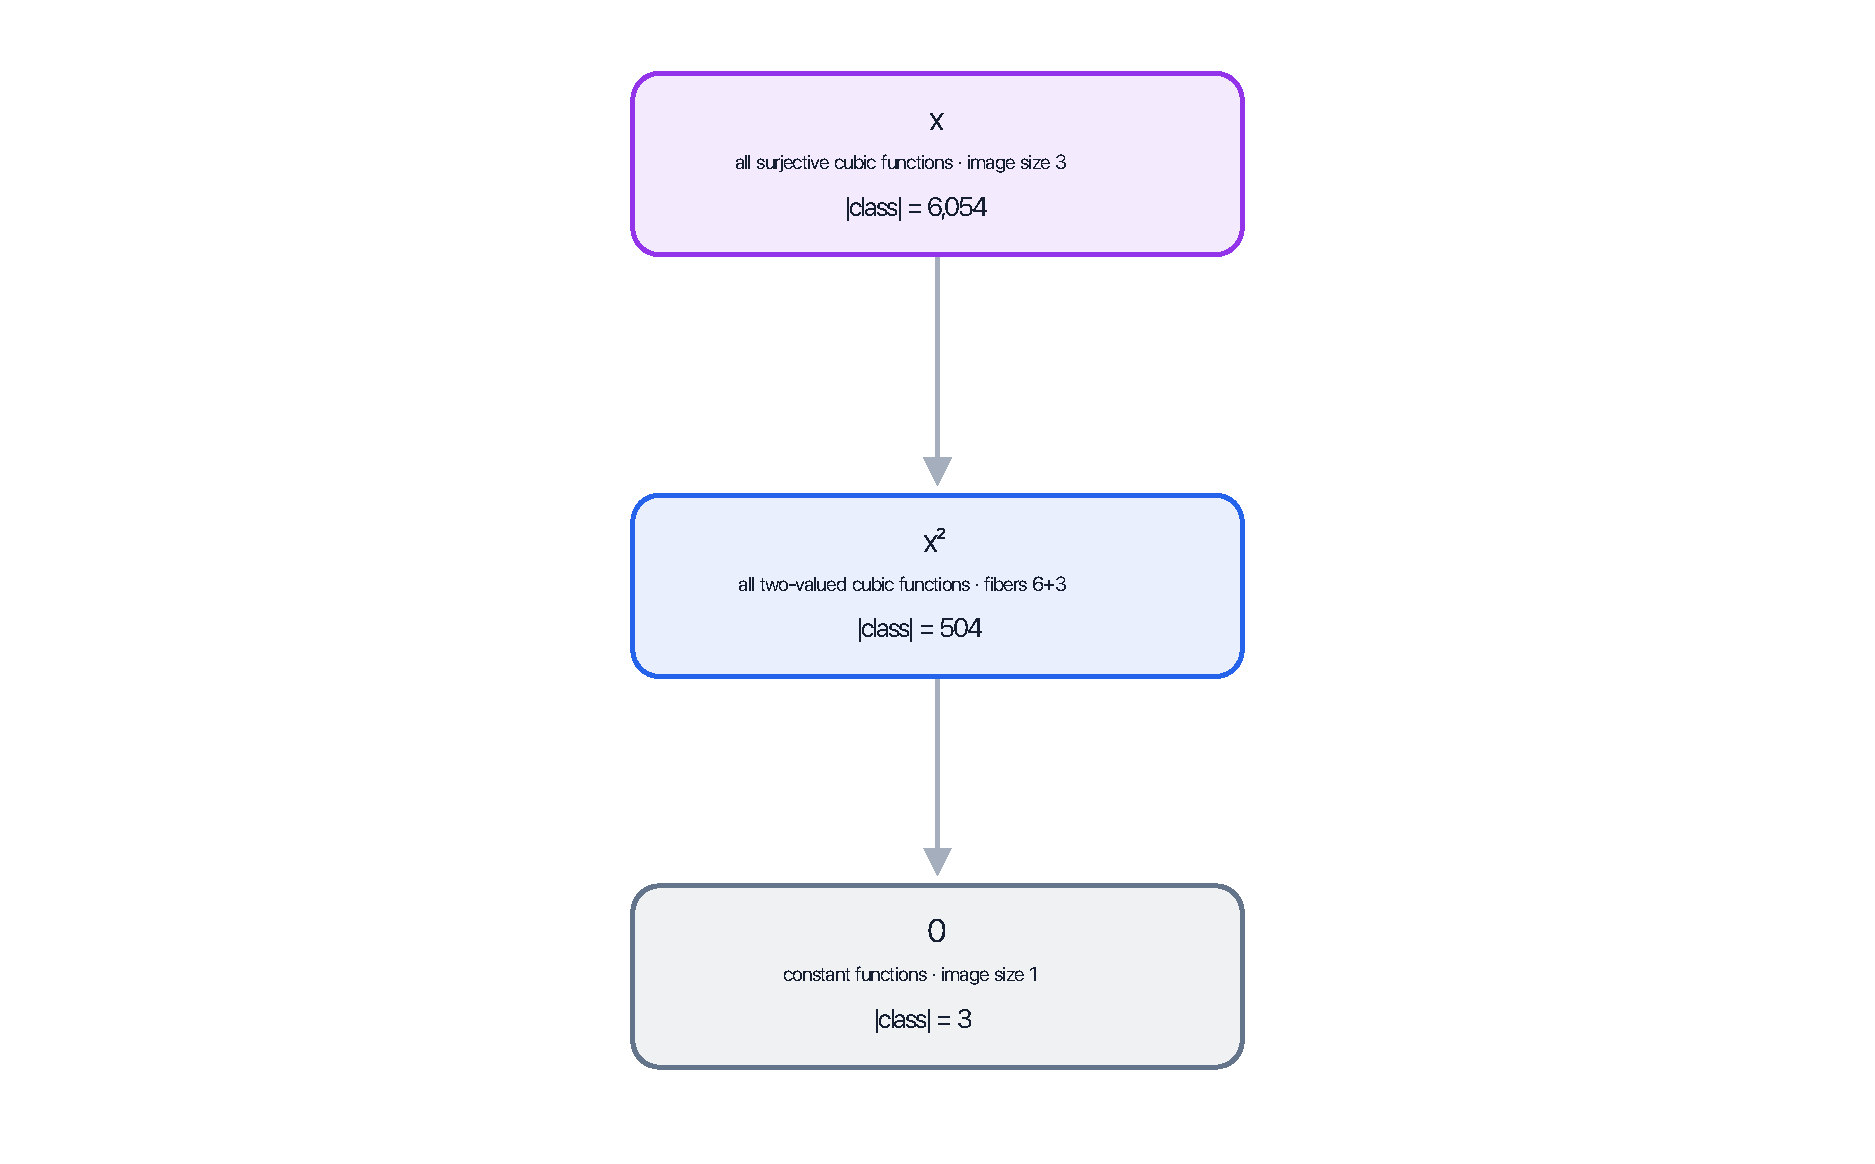
\includegraphics[width=0.78\textwidth]{figures/cubic-map-poset-q3-quadratic-input.pdf}
  \caption{The generated preorder with quadratic input and linear output
  processors: three mutual-reachability classes and two covers.  It is not a
  group-orbit classification by invertible quadratic substitutions.}
\end{figure}

\clearpage
\begin{landscape}
  \begin{figure}[p]
    \centering
    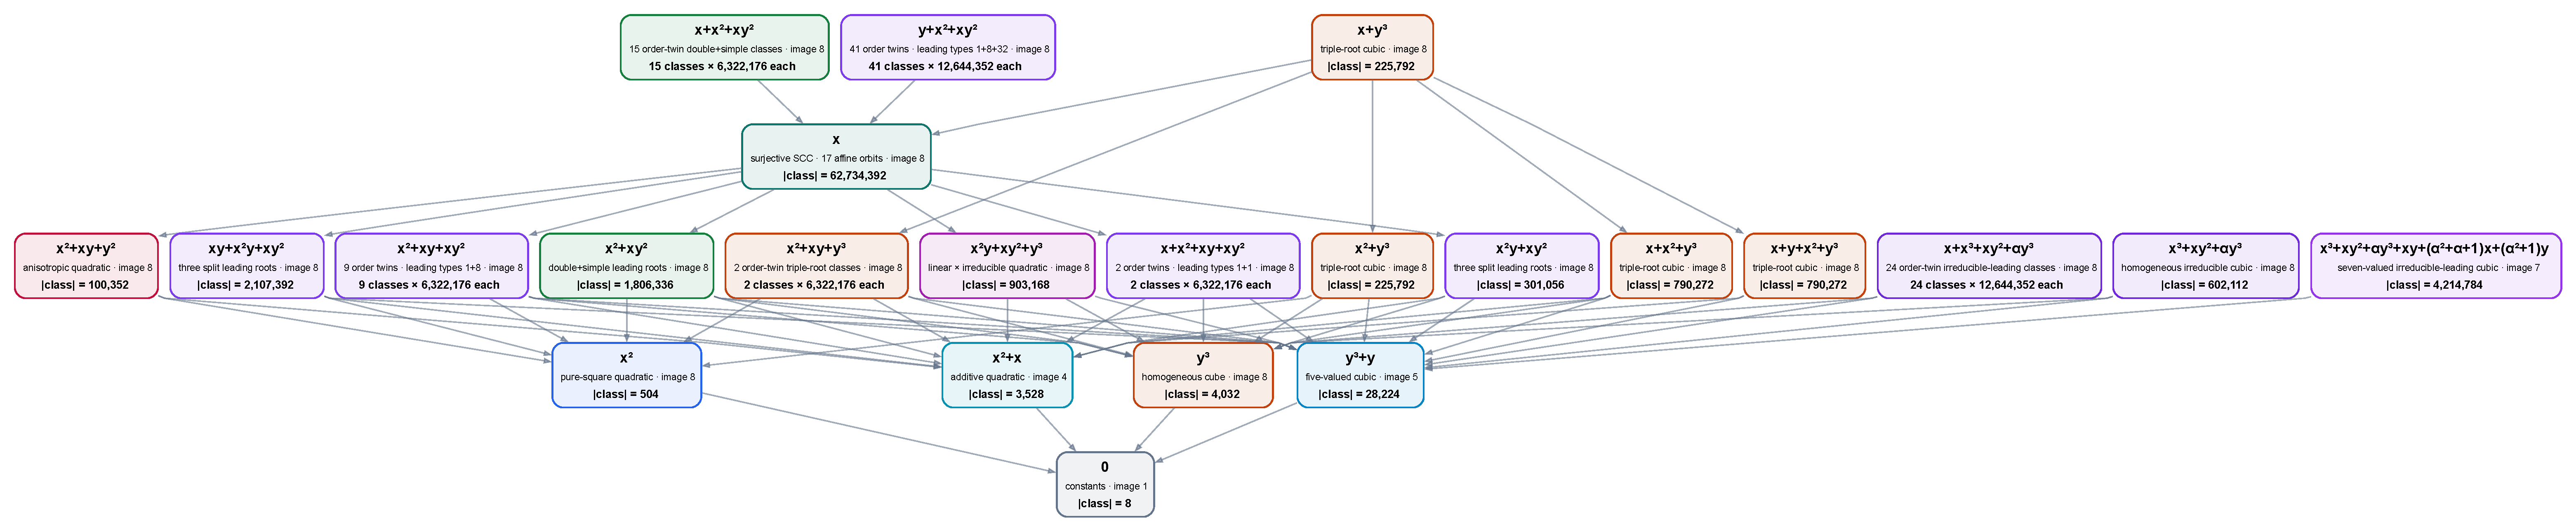
\includegraphics[width=0.98\linewidth,height=0.72\textheight,keepaspectratio]{figures/cubic-map-poset-q8-quadratic-input.pdf}
    \caption{The corresponding quadratic-input calculation over \(\F_8\):
    \(110\) classes grouped into \(23\) boxes of order-theoretic twins, with
    \(57\) covers between the boxes.  Output processors are linear.}
  \end{figure}
\end{landscape}

\section*{Code and data availability}

The diagrams, exhaustive classifiers, residue calculations, exchange-rate
library, and cycle tables are contained in the accompanying repository.  The
main regeneration commands are:
\begin{itemize}
  \item \path{cli/finite_field_map_poset_cli} for the affine quadratic atlas;
  \item \path{cli/homogeneous_tensor_poset_cli} for the homogeneous cases;
  \item \path{cli/cubic_map_poset_cli} for the cubic processor comparisons;
  \item \path{analysis/polynomial_map_exchange_examples.py} for the exchange
  matrices and cycle means used here.
\end{itemize}

\begingroup
\small
\setlength{\itemsep}{0.25em}
\begin{thebibliography}{99}

\bibitem{vorozhtsov-exchange}
A.~Vorozhtsov,
\emph{Complexity of finite maps and energy--entropy curves: exchange rates,
and a comparison that runs in circles}, companion manuscript, 2026.

\bibitem{fritz-resource}
T.~Fritz,
Resource convertibility and ordered commutative monoids,
\emph{Math. Structures Comput. Sci.} \textbf{27} (2017), 850--938,
\url{https://doi.org/10.1017/S0960129515000444}.

\bibitem{strassen-spectrum}
V.~Strassen,
The asymptotic spectrum of tensors,
\emph{J. Reine Angew. Math.} \textbf{384} (1988), 102--152,
\url{https://doi.org/10.1515/crll.1988.384.102}.

\bibitem{kerner-left-right}
D.~Kerner,
Orbits of the left--right equivalence of maps in arbitrary characteristic,
\emph{arXiv:2111.02715}, 2021,
\url{https://arxiv.org/abs/2111.02715}.

\bibitem{birkes-orbits}
D.~Birkes,
Orbits of linear algebraic groups,
\emph{Ann. of Math.} \textbf{93} (1971), 459--475,
\url{https://doi.org/10.2307/1970884}.

\bibitem{lam-quadratic}
T.~Y. Lam,
\emph{Introduction to Quadratic Forms over Fields},
Graduate Studies in Mathematics 67, American Mathematical Society, 2005.

\bibitem{lidl-finite-fields}
R.~Lidl and H.~Niederreiter,
\emph{Finite Fields}, second edition,
Encyclopedia of Mathematics and its Applications 20,
Cambridge University Press, 1997.

\bibitem{serre-arithmetic}
J.-P. Serre,
\emph{A Course in Arithmetic},
Graduate Texts in Mathematics 7, Springer, 1973.

\bibitem{karp-cycle-mean}
R.~M. Karp,
A characterization of the minimum cycle mean in a digraph,
\emph{Discrete Math.} \textbf{23} (1978), 309--311,
\url{https://doi.org/10.1016/0012-365X(78)90011-0}.

\bibitem{igusa-zeta}
J.-I. Igusa,
Complex powers and asymptotic expansions. I. Functions of certain types,
\emph{J. Reine Angew. Math.} \textbf{268/269} (1974), 110--130.

\bibitem{bost-connes}
J.-B. Bost and A.~Connes,
Hecke algebras, type III factors and phase transitions with spontaneous
symmetry breaking in number theory,
\emph{Selecta Math.} \textbf{1} (1995), 411--457,
\url{https://doi.org/10.1007/BF01589495}.

\bibitem{tate-thesis}
J.~Tate,
Fourier analysis in number fields and Hecke's zeta-functions,
in J.~W.~S. Cassels and A.~Fr\"ohlich (eds.),
\emph{Algebraic Number Theory}, Academic Press, 1967, pp.~305--347.

\bibitem{weil-explicit}
A.~Weil,
Sur les ``formules explicites'' de la th\'eorie des nombres premiers,
\emph{Comm. S\'em. Math. Univ. Lund, Tome Suppl.} (1952), 252--265.

\bibitem{berry-keating}
M.~V. Berry and J.~P. Keating,
The Riemann zeros and eigenvalue asymptotics,
\emph{SIAM Rev.} \textbf{41} (1999), 236--266,
\url{https://doi.org/10.1137/S0036144598347497}.

\end{thebibliography}
\endgroup

\end{document}
